\documentclass[]{beamer} 
\usetheme{Copenhagen}
\usecolortheme{default}

\usepackage[latin1]{inputenc}
\usepackage{graphicx}
\usepackage{amsmath}
\usepackage{verbatim}
\usepackage{subfigure}
\usepackage{hyperref}

\title{$B_{s}\to D_{s}K\pi\pi$ : $\gamma$ measurement}
\author{Philippe d'Argent \inst{1}, Evelina Gersabeck \inst{1}, \underline{Matthieu Kecke} \inst{1}, Manuel Schiller \inst{2}}
\institute{\inst{1} PI Heidelberg, \inst{2} Glasgow}
\date{xx.xx.2017}
\setbeamertemplate{footline}[page number]
\begin{document}
\frame{\titlepage}


\begin{frame}
\frametitle{Status}

A lot of progress since last update:

\begin{itemize}

\item re-optimized selection for $\gamma$ measurement

\item added 2015 \& 2016 Run2 data 

\item use Meerkat PID sampling to control misID contributions

\item developed time dependent MINT version 

\item integrated time acceptance and resolution in TD-MINT

\item New MC request, a lot more statistics needed 

\end{itemize}


\end{frame}


\begin{frame}
\frametitle{Re-optimized Selection}

We now use specific phasespace cuts during preselection to suppress background:  

plot here

\[m(K\pi\pi) < xXx GeV\]

The reduced background level allows us to loosen the BDT cut and significantly improve $\frac{S}{\sqrt{S+B}}$ 


\end{frame}

\begin{frame}
\frametitle{New data!}

Data from 2015 \& 2016 now added to analysis \newline

Slightly reorganized mass fits, now fit simultaneously in every year and $D_{s}$ final state:

\begin{itemize} 

\item years: 2011, 2012, 2015, 2016

\item $D_{s}\to \phi\pi \to KK\pi$

\item $D_{s}\to K^{*}K \to KK\pi$

\item $D_{s} \to KK\pi$ (non-resonant)

\item $D_{s} \to \pi\pi\pi$

\end{itemize}

\end{frame}

\begin{frame}
\frametitle{Fit components}

Components we model in the invariant mass distributions:\newline

$B_{s}\to D_{s}\pi\pi\pi$ :

\begin{itemize}

 \item $B_{s}$ signal

 \item  $B_{s}\to D_{s}^{*}\pi\pi\pi$ partial reconstructed background combinatorial

\item combinatorial background

\end{itemize}



$B_{s}\to D_{s}K\pi\pi$ :

\begin{itemize}

\item $B_{s}/B^{0}$ signal

\item  $B_{s}/B^{0}\to D_{s}^{*}K\pi\pi$ partial reconstructed background

\item  $B_{s}\to D_{s}\pi\pi\pi$ mis-ID background

\item combinatorial background 

\end{itemize}


\end{frame}

\begin{frame}
\frametitle{Massfits norm 15}

\begin{figure}[h]
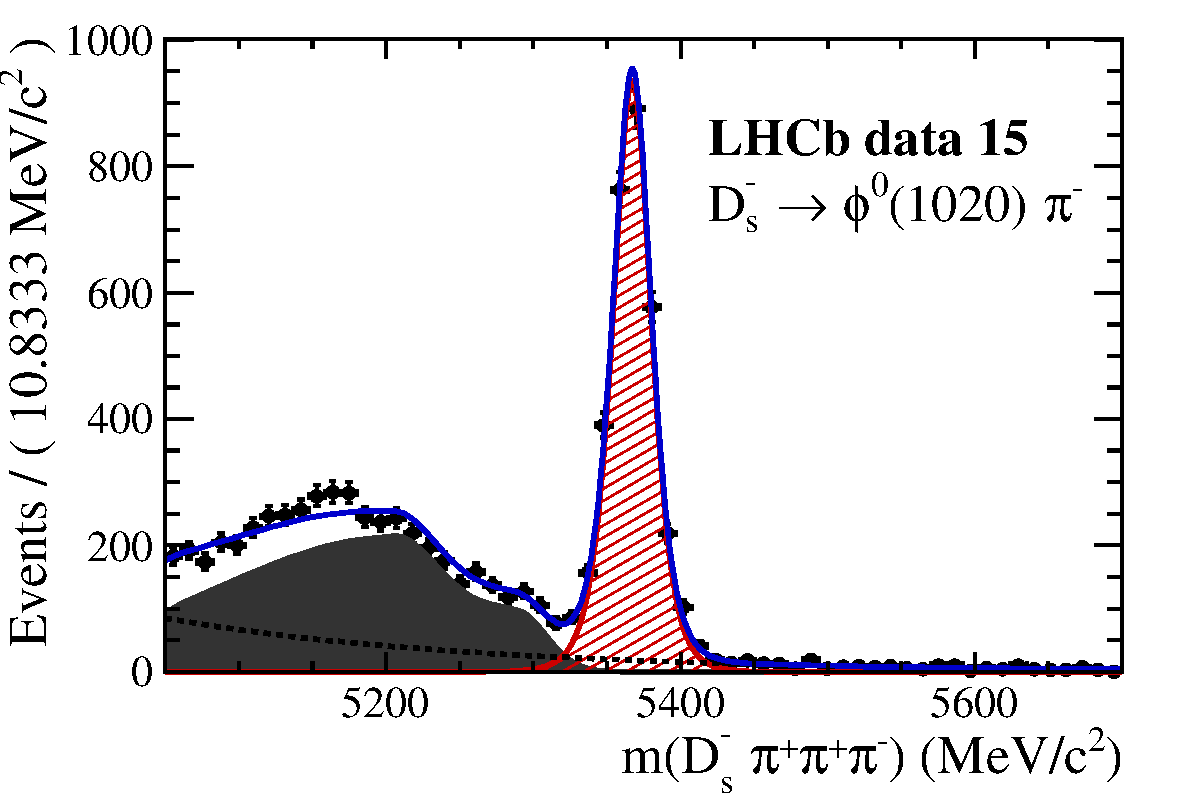
\includegraphics[height=!,width=0.5\textwidth]{plots/norm_y15_phipi.pdf}
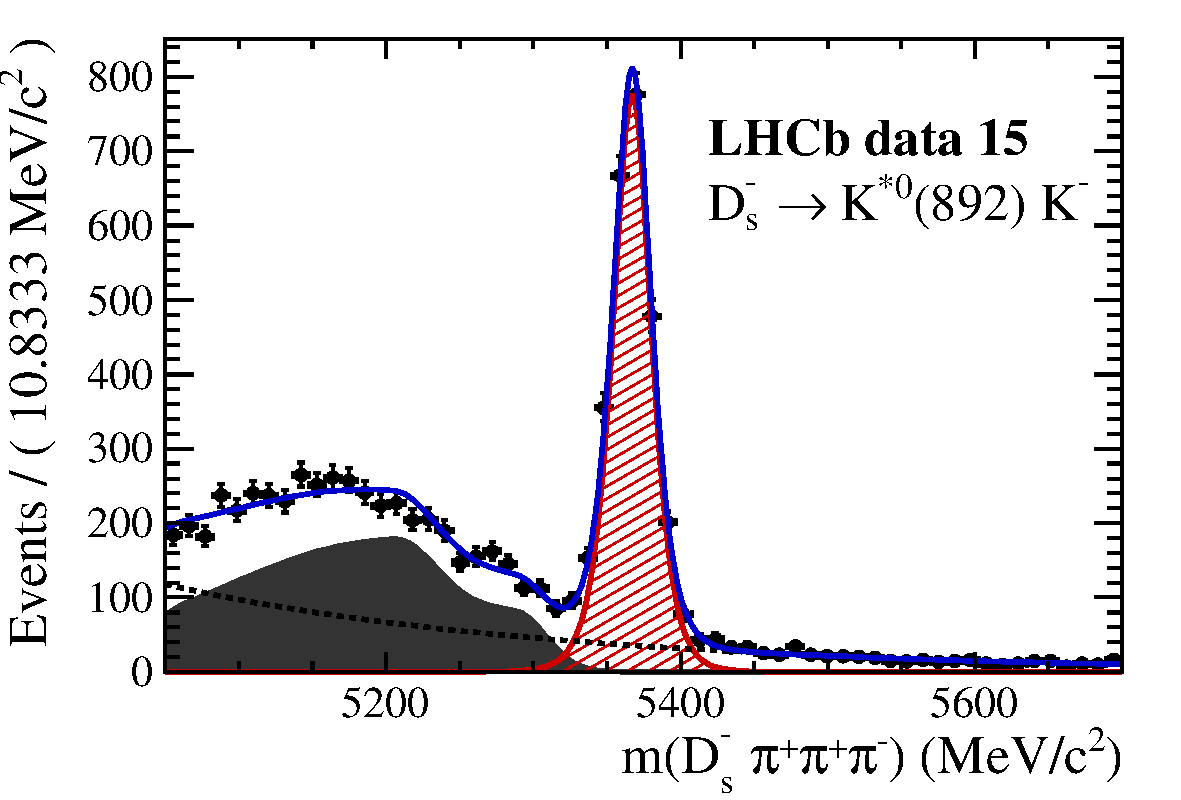
\includegraphics[height=!,width=0.5\textwidth]{plots/norm_y15_KsK.pdf}\\
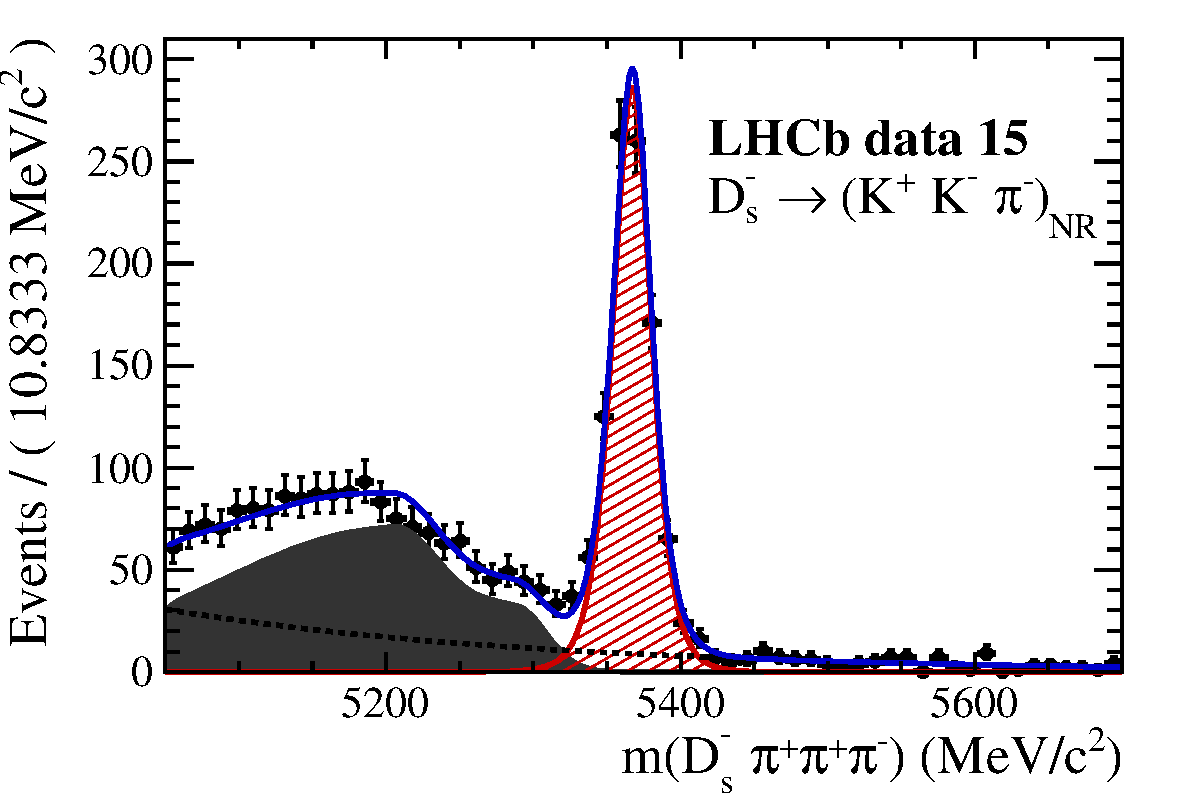
\includegraphics[height=!,width=0.5\textwidth]{plots/norm_y15_KKpi_NR.pdf}
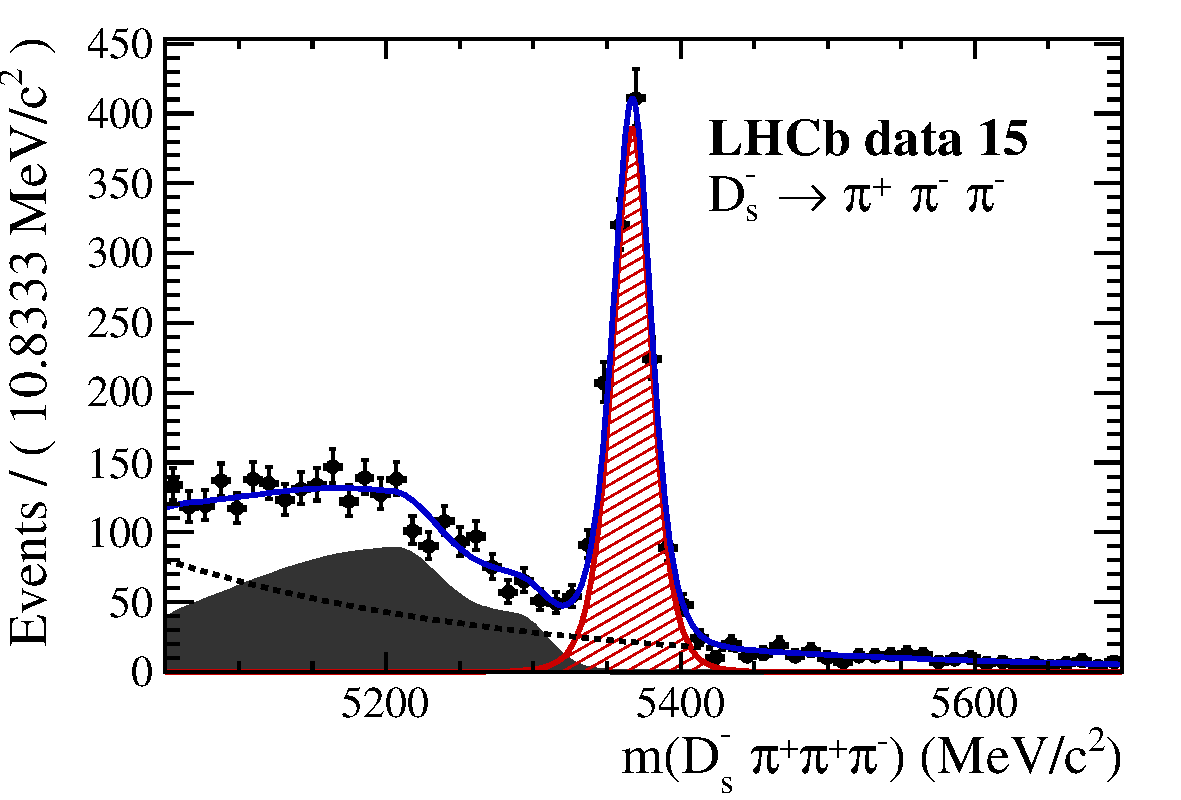
\includegraphics[height=!,width=0.5\textwidth]{plots/norm_y15_pipipi.pdf}
\end{figure}

\end{frame}

\begin{frame}
\frametitle{Massfits norm 16}

\begin{figure}
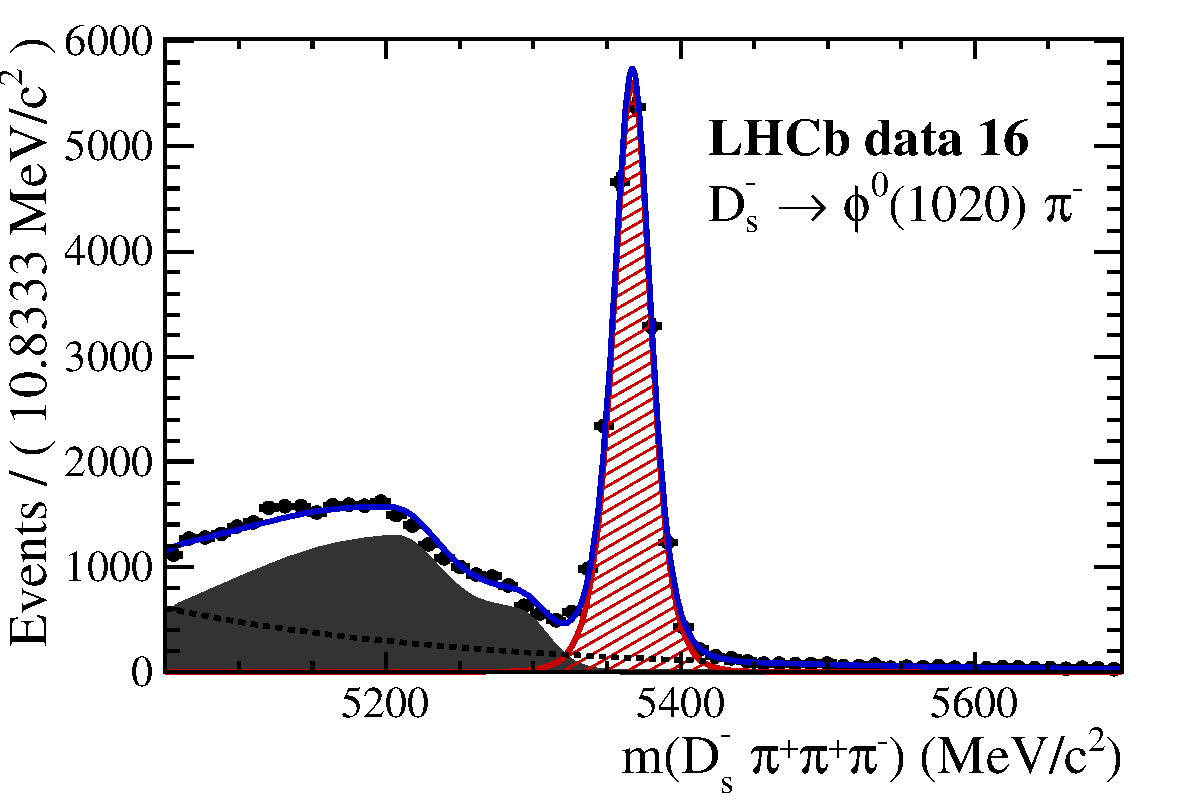
\includegraphics[height=!,width=0.5\textwidth]{plots/norm_y16_phipi.pdf}
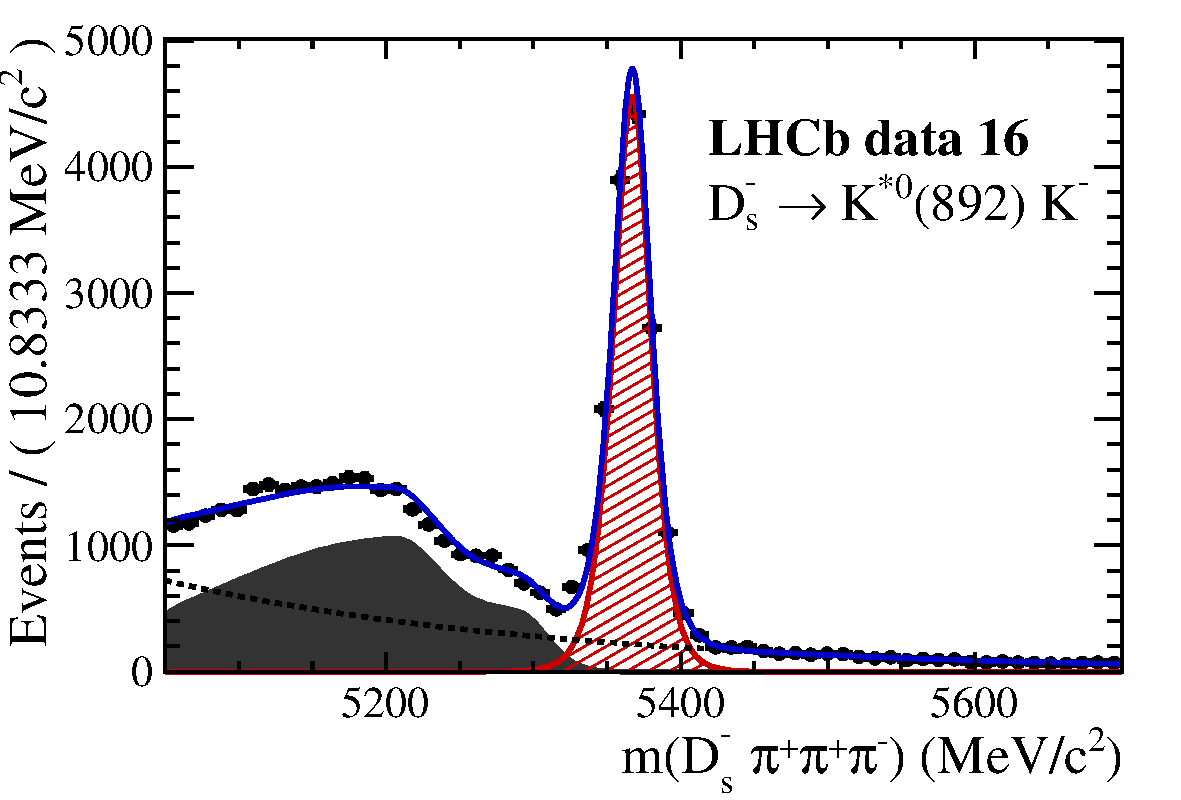
\includegraphics[height=!,width=0.5\textwidth]{plots/norm_y16_KsK.pdf}\\
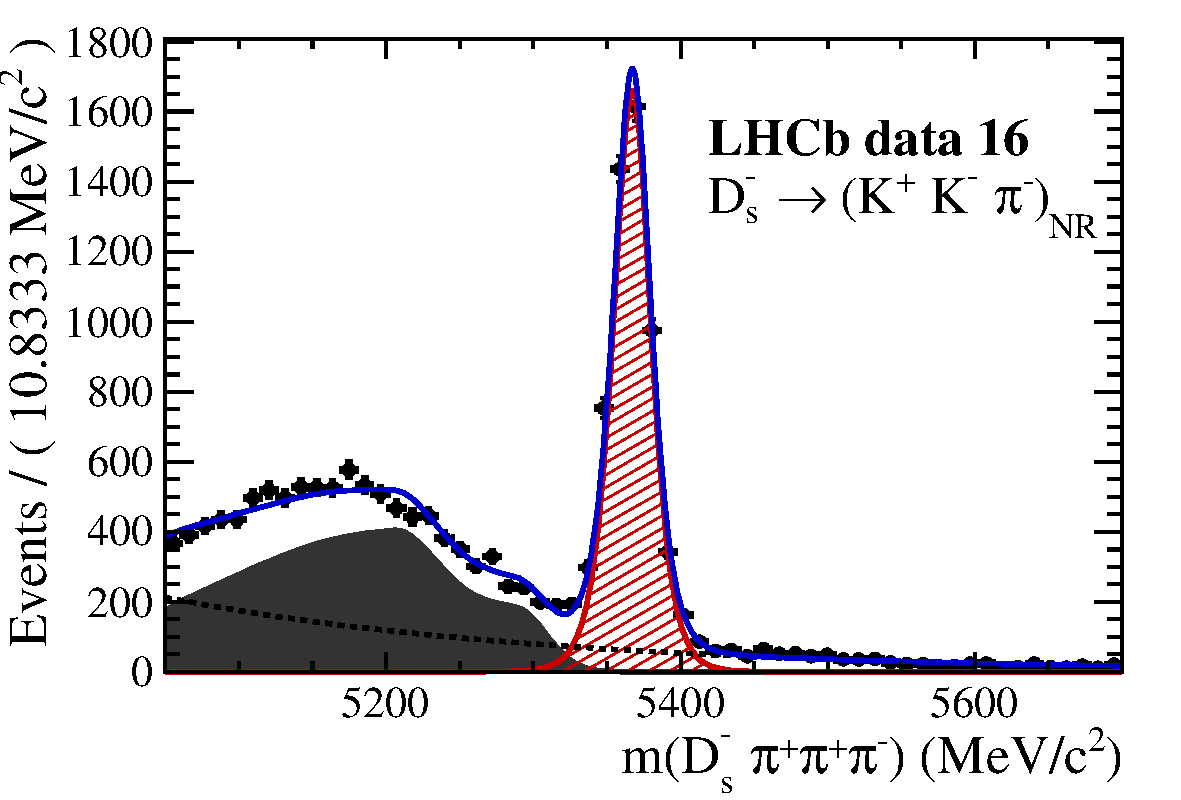
\includegraphics[height=!,width=0.5\textwidth]{plots/norm_y16_KKpi_NR.pdf}
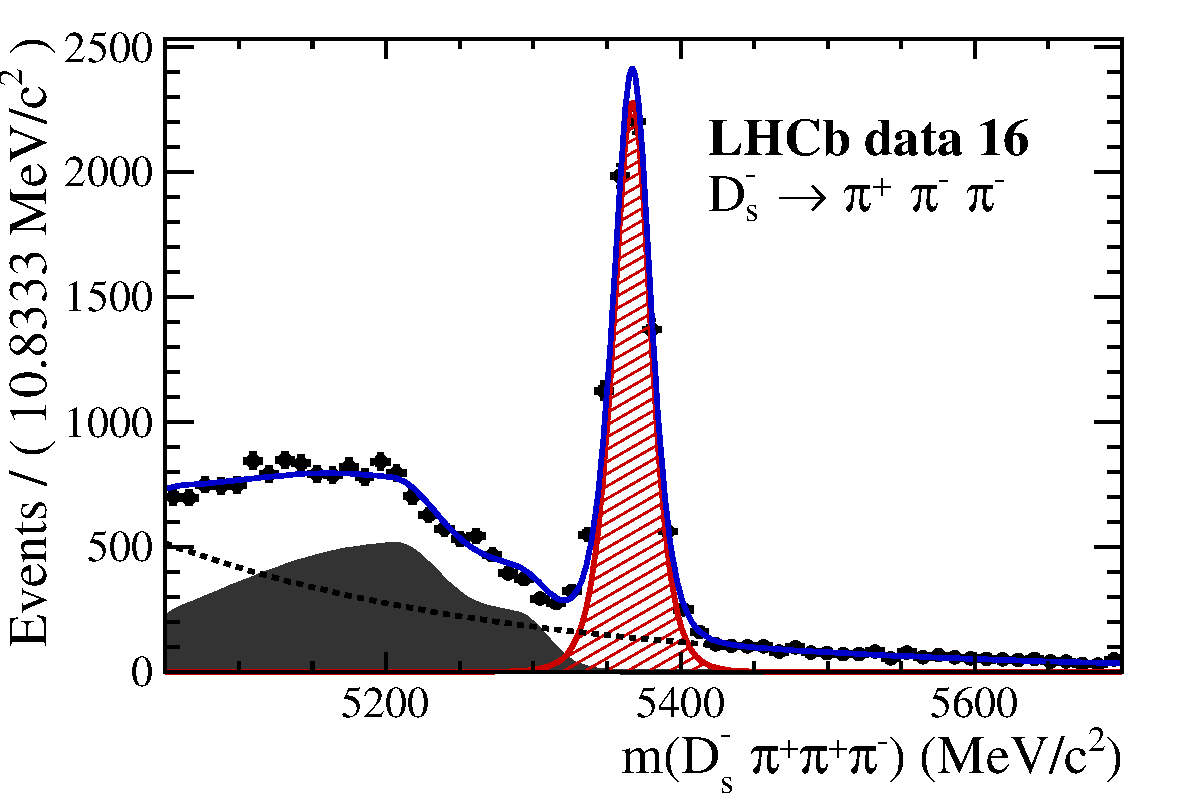
\includegraphics[height=!,width=0.5\textwidth]{plots/norm_y16_pipipi.pdf}
\end{figure}

\end{frame}

\begin{frame}
\frametitle{Massfits signal 15}

\begin{figure}[h]
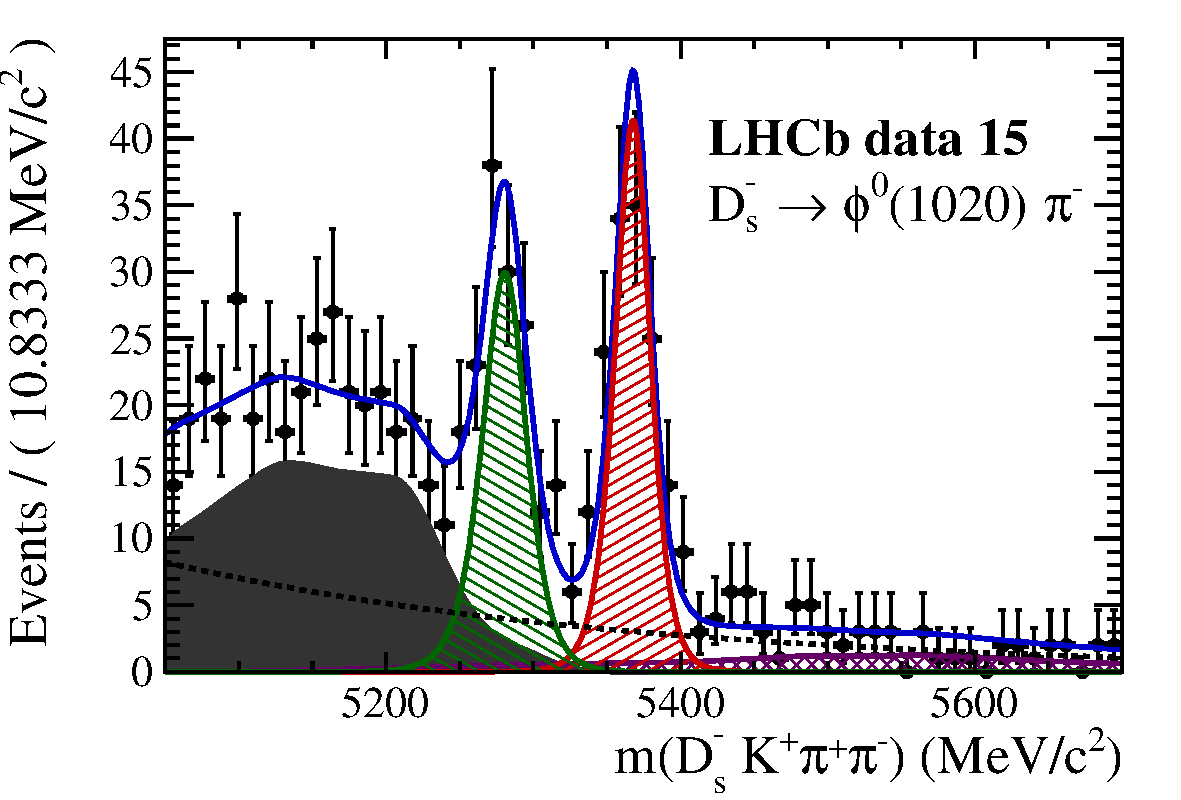
\includegraphics[height=!,width=0.5\textwidth]{plots/signal_y15_phipi.pdf}
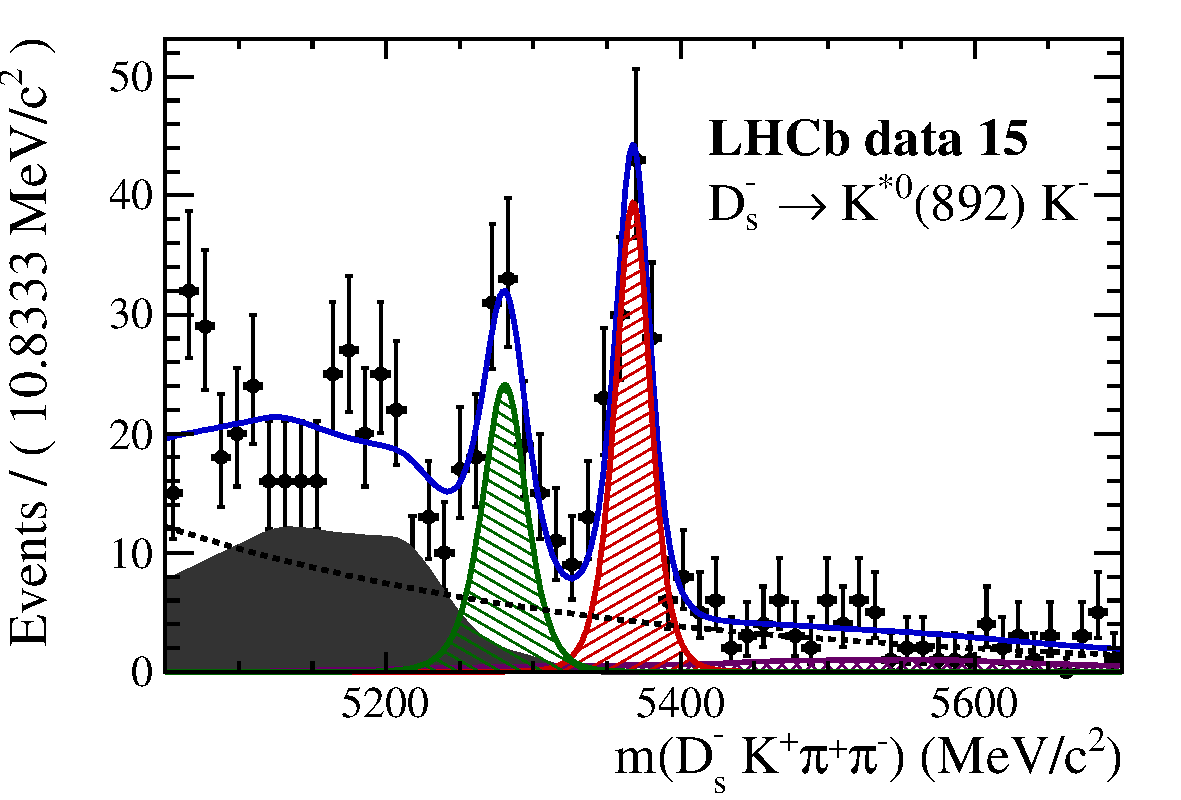
\includegraphics[height=!,width=0.5\textwidth]{plots/signal_y15_KsK.pdf}\\
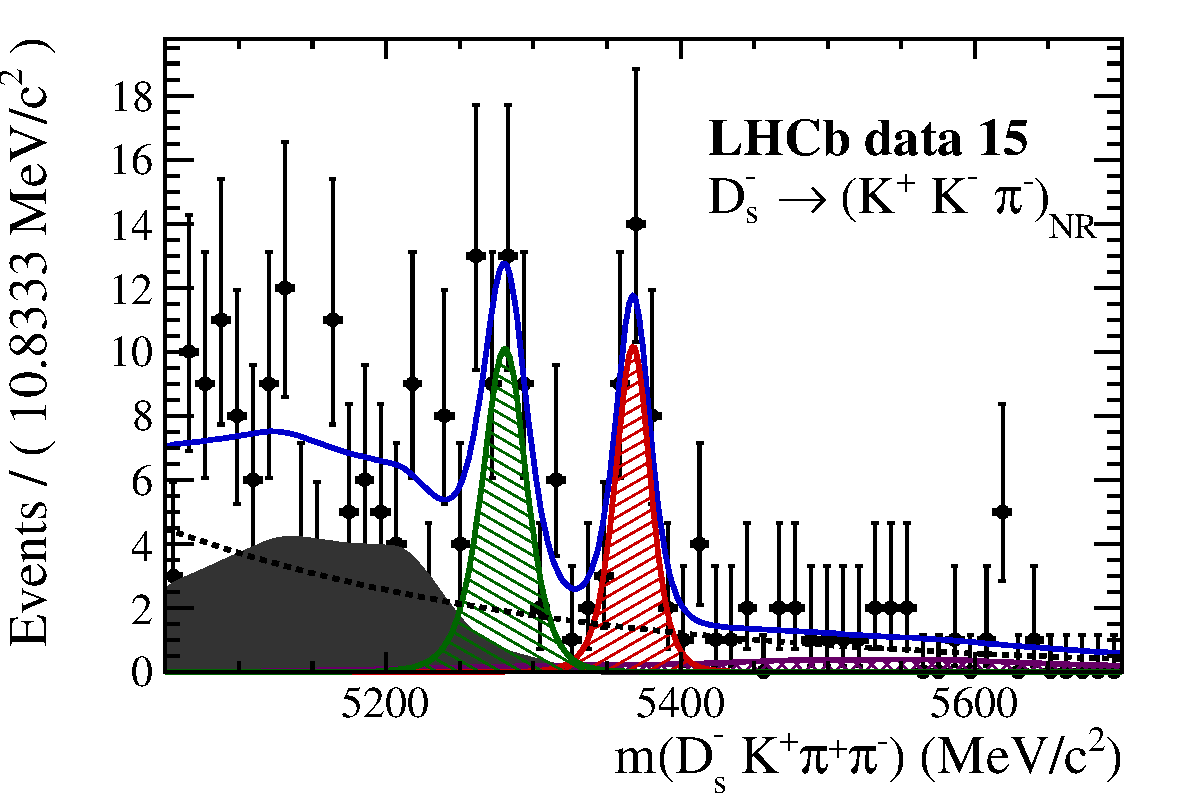
\includegraphics[height=!,width=0.5\textwidth]{plots/signal_y15_KKpi_NR.pdf}
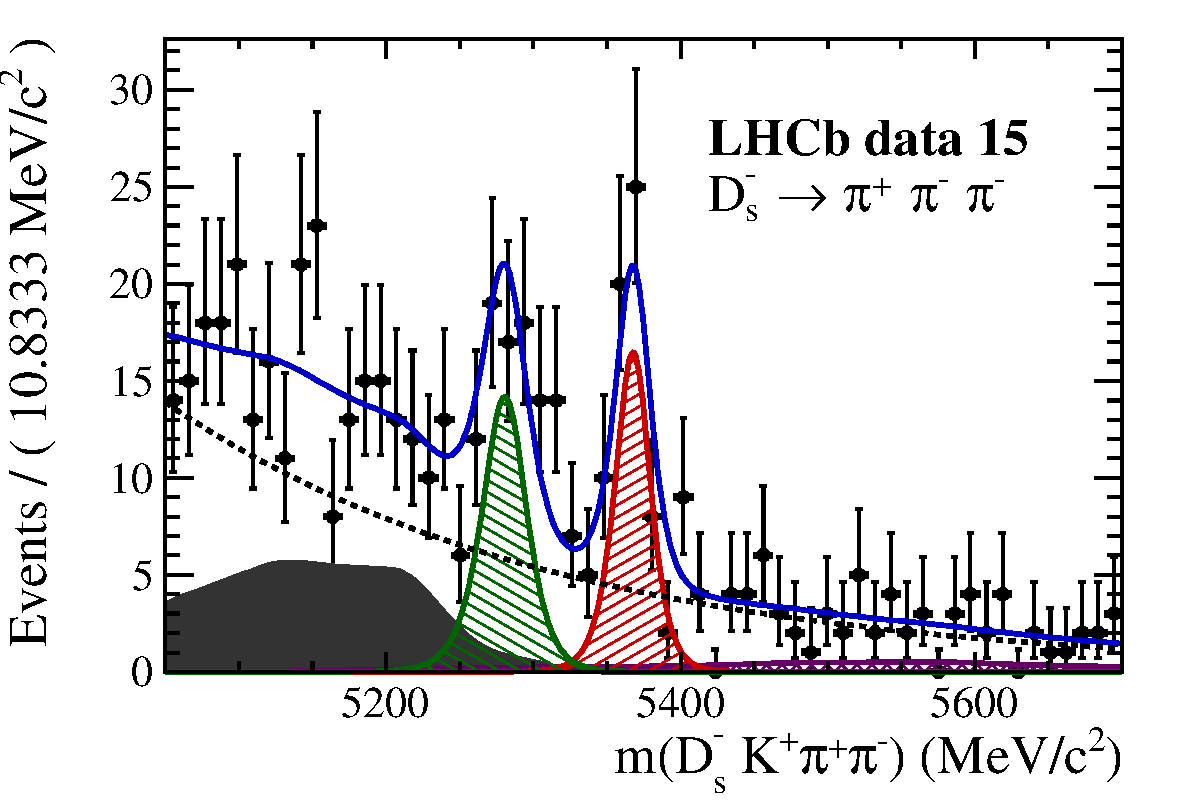
\includegraphics[height=!,width=0.5\textwidth]{plots/signal_y15_pipipi.pdf}
\end{figure}

\end{frame}

\begin{frame}
\frametitle{Massfits signal 16}

\begin{figure}
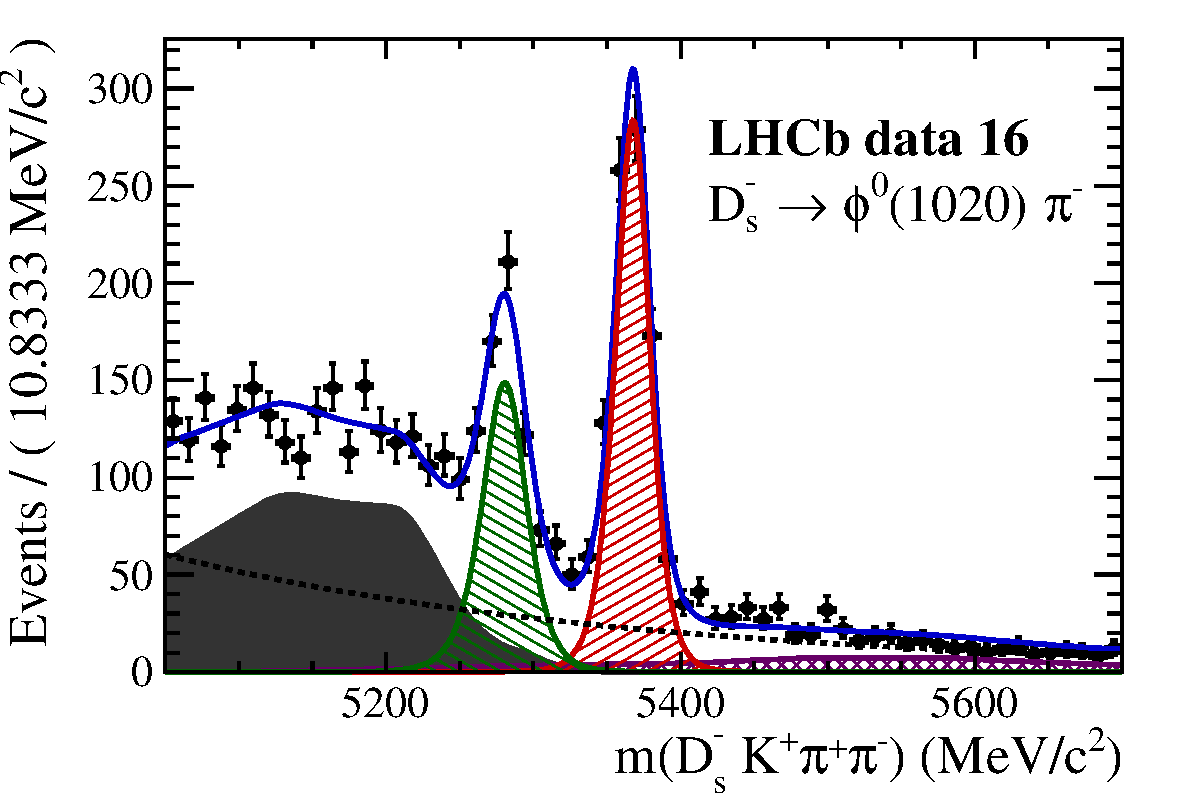
\includegraphics[height=!,width=0.5\textwidth]{plots/signal_y16_phipi.pdf}
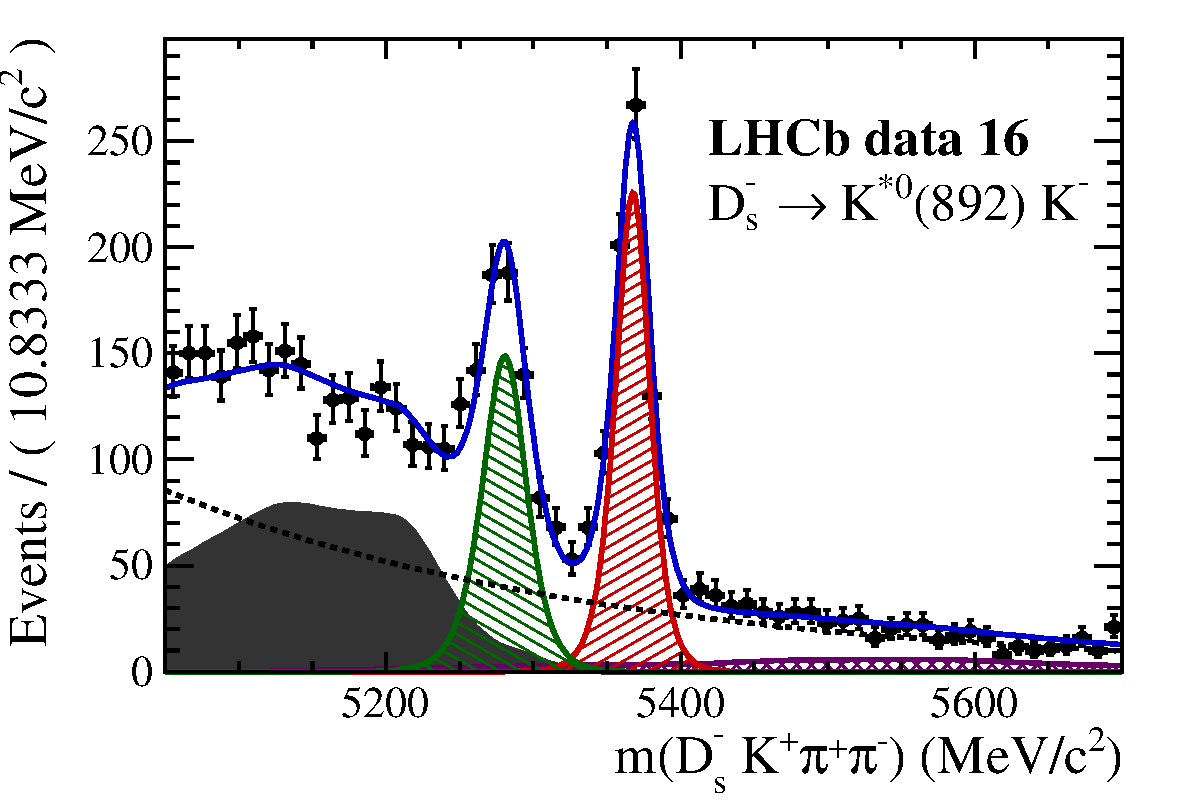
\includegraphics[height=!,width=0.5\textwidth]{plots/signal_y16_KsK.pdf}\\
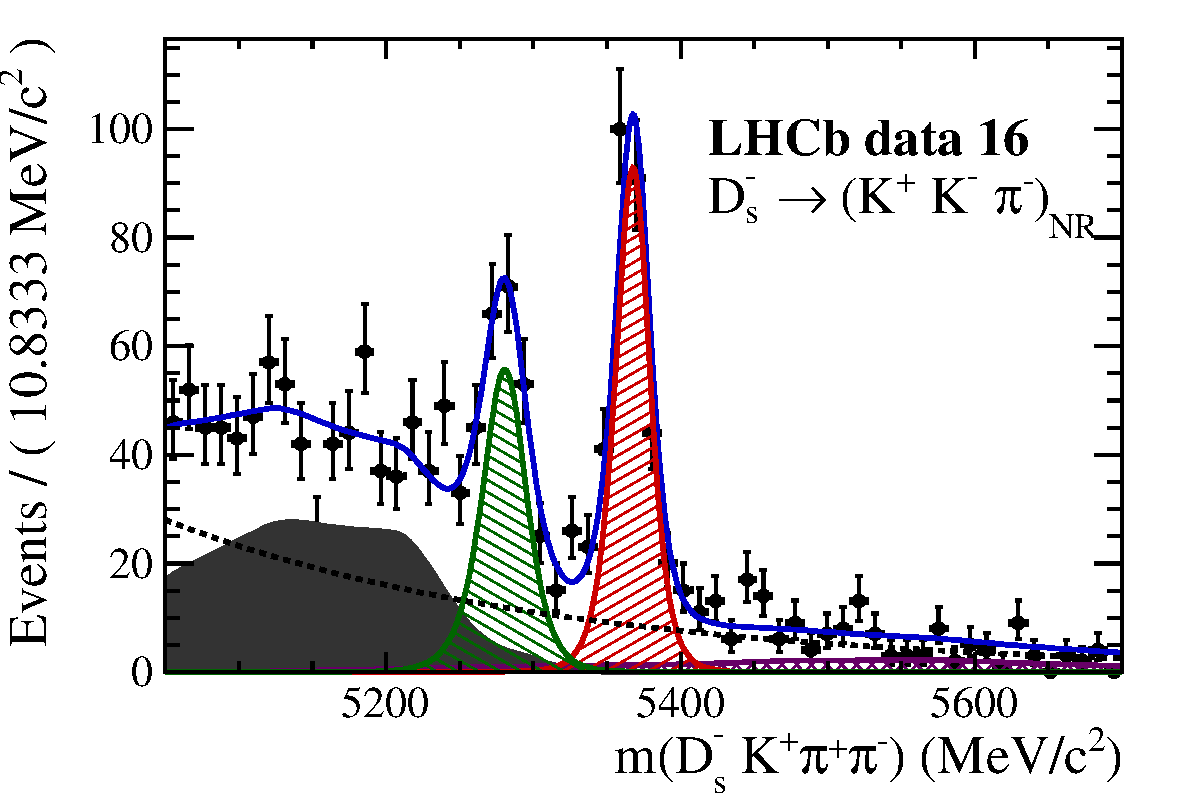
\includegraphics[height=!,width=0.5\textwidth]{plots/signal_y16_KKpi_NR.pdf}
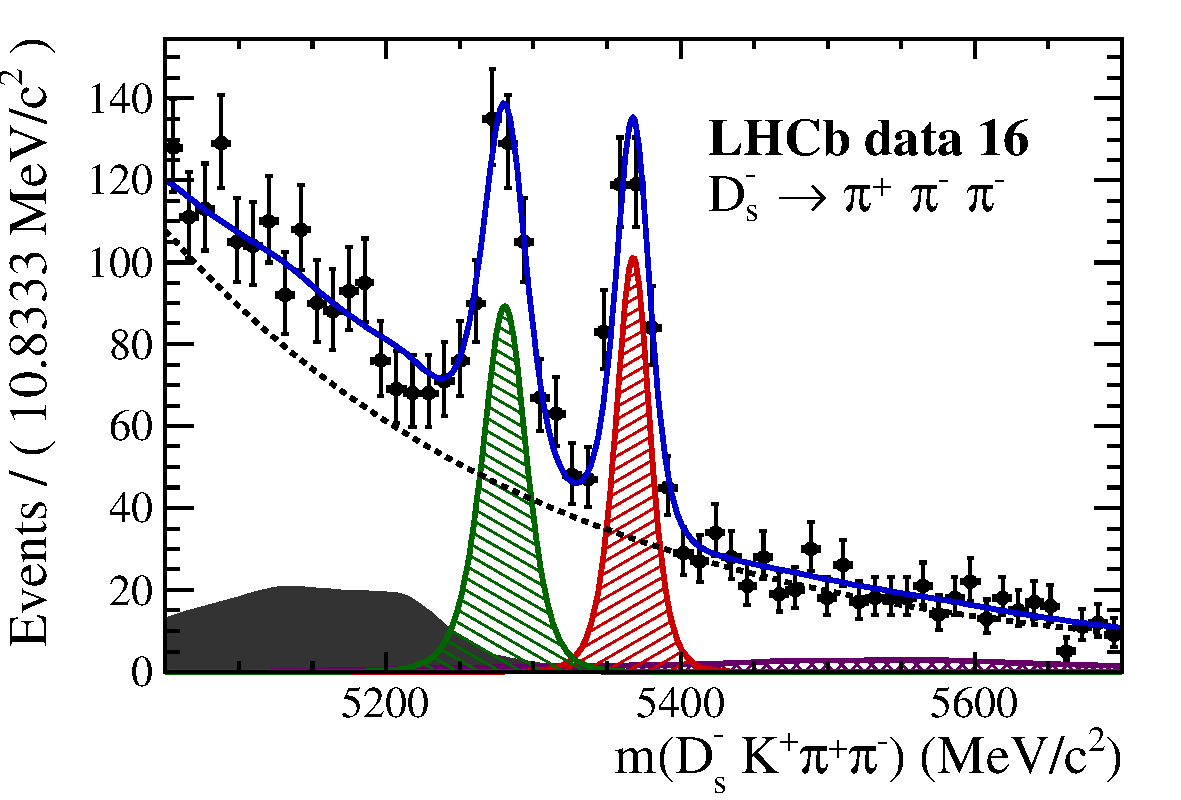
\includegraphics[height=!,width=0.5\textwidth]{plots/signal_y16_pipipi.pdf}
\end{figure}


\end{frame}

\begin{frame}
\frametitle{Run1 \& 2 Data combined}

\begin{figure}
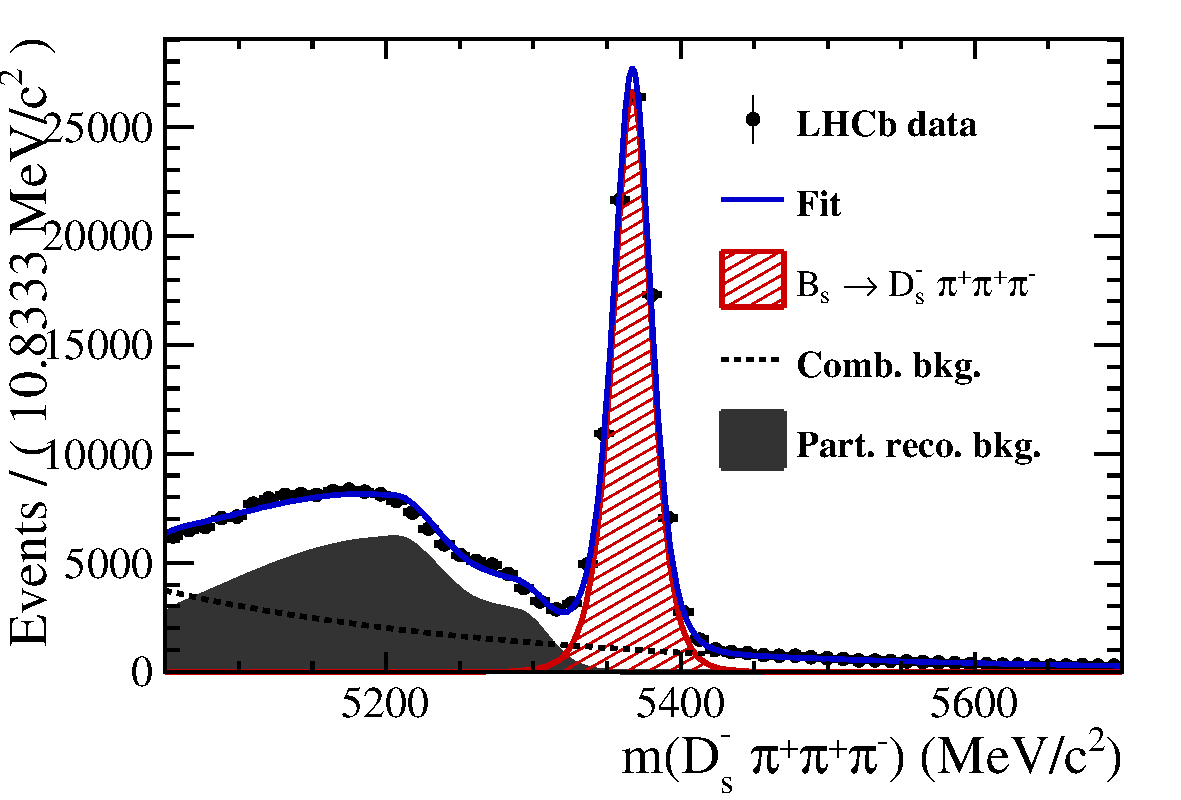
\includegraphics[width=0.49\textwidth, height = 5.cm]{plots/norm.pdf}
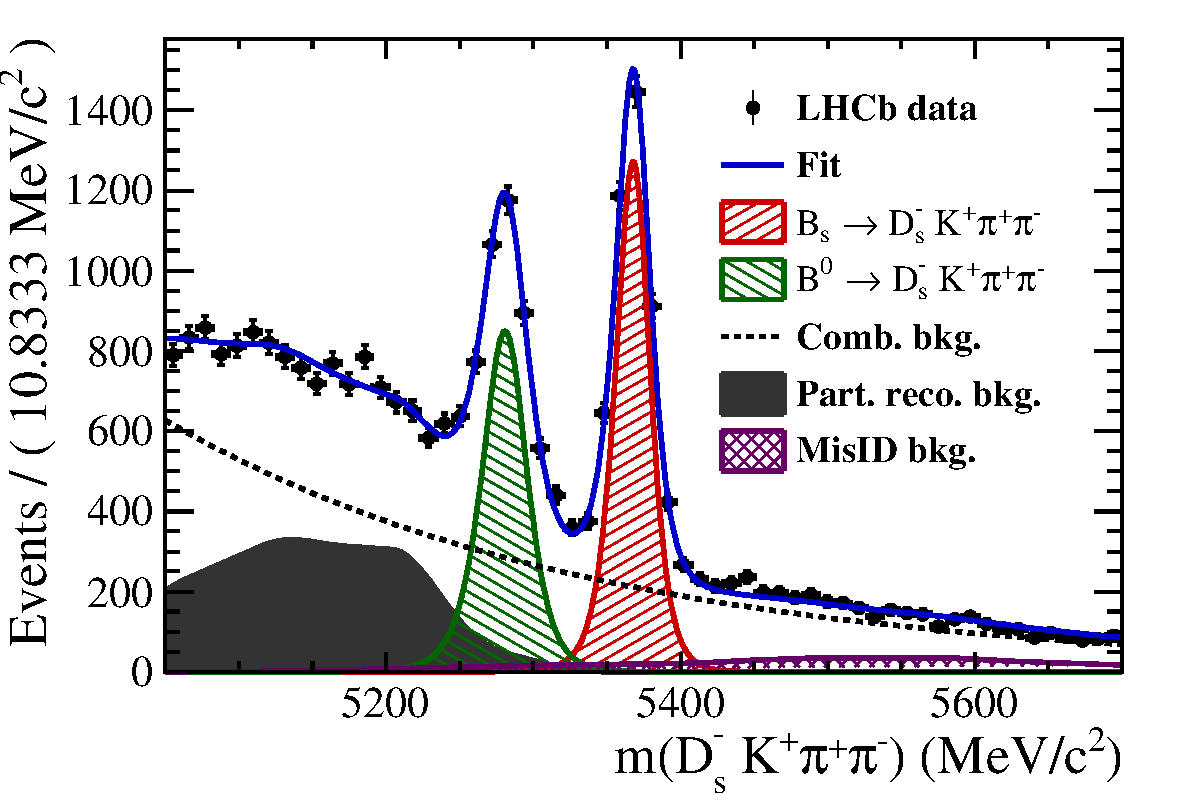
\includegraphics[width=0.49\textwidth, height = 5.cm]{plots/signal.pdf}
\end{figure}

\small

\begin{table}
\centering
 \begin{tabular}{l || l l l l}
fit component & yield 2011 & yield 2012 & yield 2015 & yield 2016\ \\
\hline \hline
$B_{s}\to D_{s}\pi\pi\pi$ & 9554 $\pm$ 204 & 22940 $\pm$ 316 & 7839 $\pm$ 185 & 45186 $\pm$ 452 \\
\hline
$B_{s}\to D_{s}K\pi\pi$ & 426 $\pm$ 57 & 909 $\pm$ 71 & 319 $\pm$ 38 & 2049 $\pm$ 104 \\
\hline
\end{tabular}
\end{table}

\normalsize

$\rightarrow$ 3700 Signals in total ! 


\end{frame}


\begin{frame}
\frametitle{Time-Acceptance}


\begin{itemize}

\item $\frac{\Gamma(t)^{observed}}{dt} = \frac{\Gamma(t)^{theory}}{dt} \cdot \epsilon(t)$

\item Use control channel $B_{s}^{0}\to D_{s}^{+}\pi^{-}\pi^{+}\pi^{-}$ 

\item describe $\epsilon(t)$ using cubic splines

\item fit flavour averaged t-distribution, e.g. \[\mathcal{P}(t^{'},\vec{\lambda}) = \left[ (e^{\Gamma_{s}t}\cdot cosh(\frac{\Delta\Gamma_{s}t}{2}) \times \mathcal{R}(t - t^{'})\right] \cdot \epsilon(t^{'}, \vec{\lambda})\]

\item fix $\Delta\Gamma$ and $\Gamma$ to PDG, float polynomials

\end{itemize} 

\end{frame}


\begin{frame}
\frametitle{Time-Acceptance}

\begin{figure}[h]
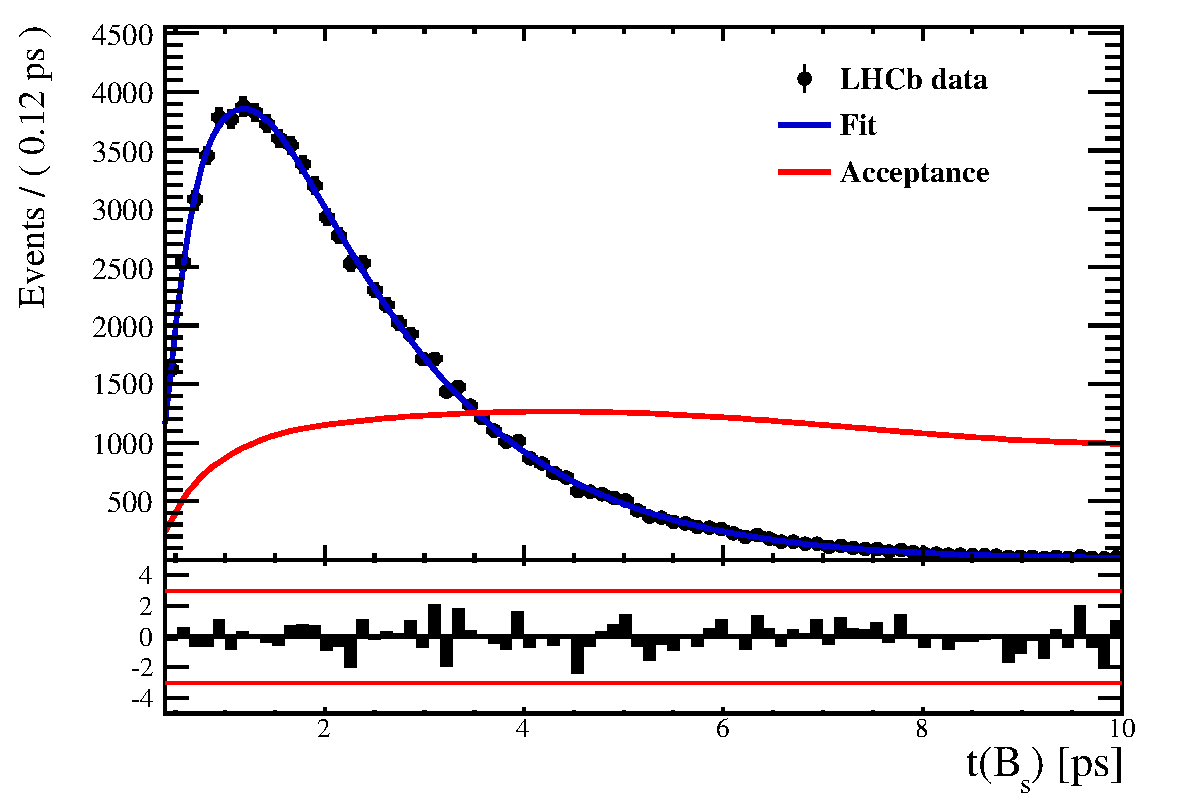
\includegraphics[width=0.8\textwidth,height=5.7cm]{plots/timeAccFit_test.pdf}
\end{figure}

knots at 0.5, 1, 1.5, 2, 3, 6. 9.5, 10 ps

\end{frame}

\begin{frame}
\frametitle{Spline Products}

\begin{figure}[h]
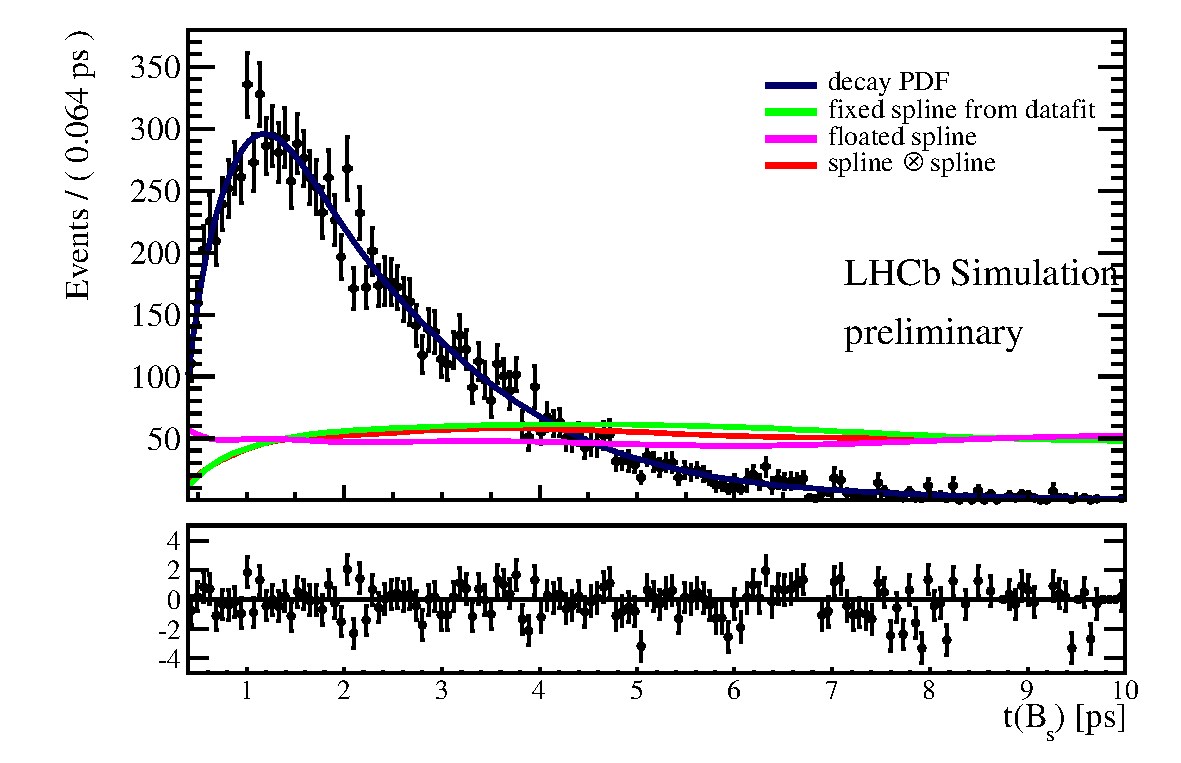
\includegraphics[width=0.8\textwidth,height=5.7cm]{plots/timeAccFit_MC_Norm_default.pdf}
\end{figure}

We also imported the Spline Product class \textcolor{blue}{\href{https://indico.cern.ch/event/606600/contributions/2692163/attachments/1508860/2352208/2017-08-16-DsK-SplineProduct.pdf}{(see talk by Agnieszka)}} to check corrections between $B_{s}\to D_{s} \pi\pi\pi$ and $B_{s}\to D_{s} K\pi\pi$ \newline

need more MC statistic for this fit

\end{frame}

\begin{frame}
\frametitle{Resolution}

Per-event decay-time error $\sigma_{t}$ estimated by the decay tree fitter \newline

Problem: Not calibrated, real decay-time error will be shifted


\begin{columns}

\column{.55\textwidth}

 \begin{figure}[h]
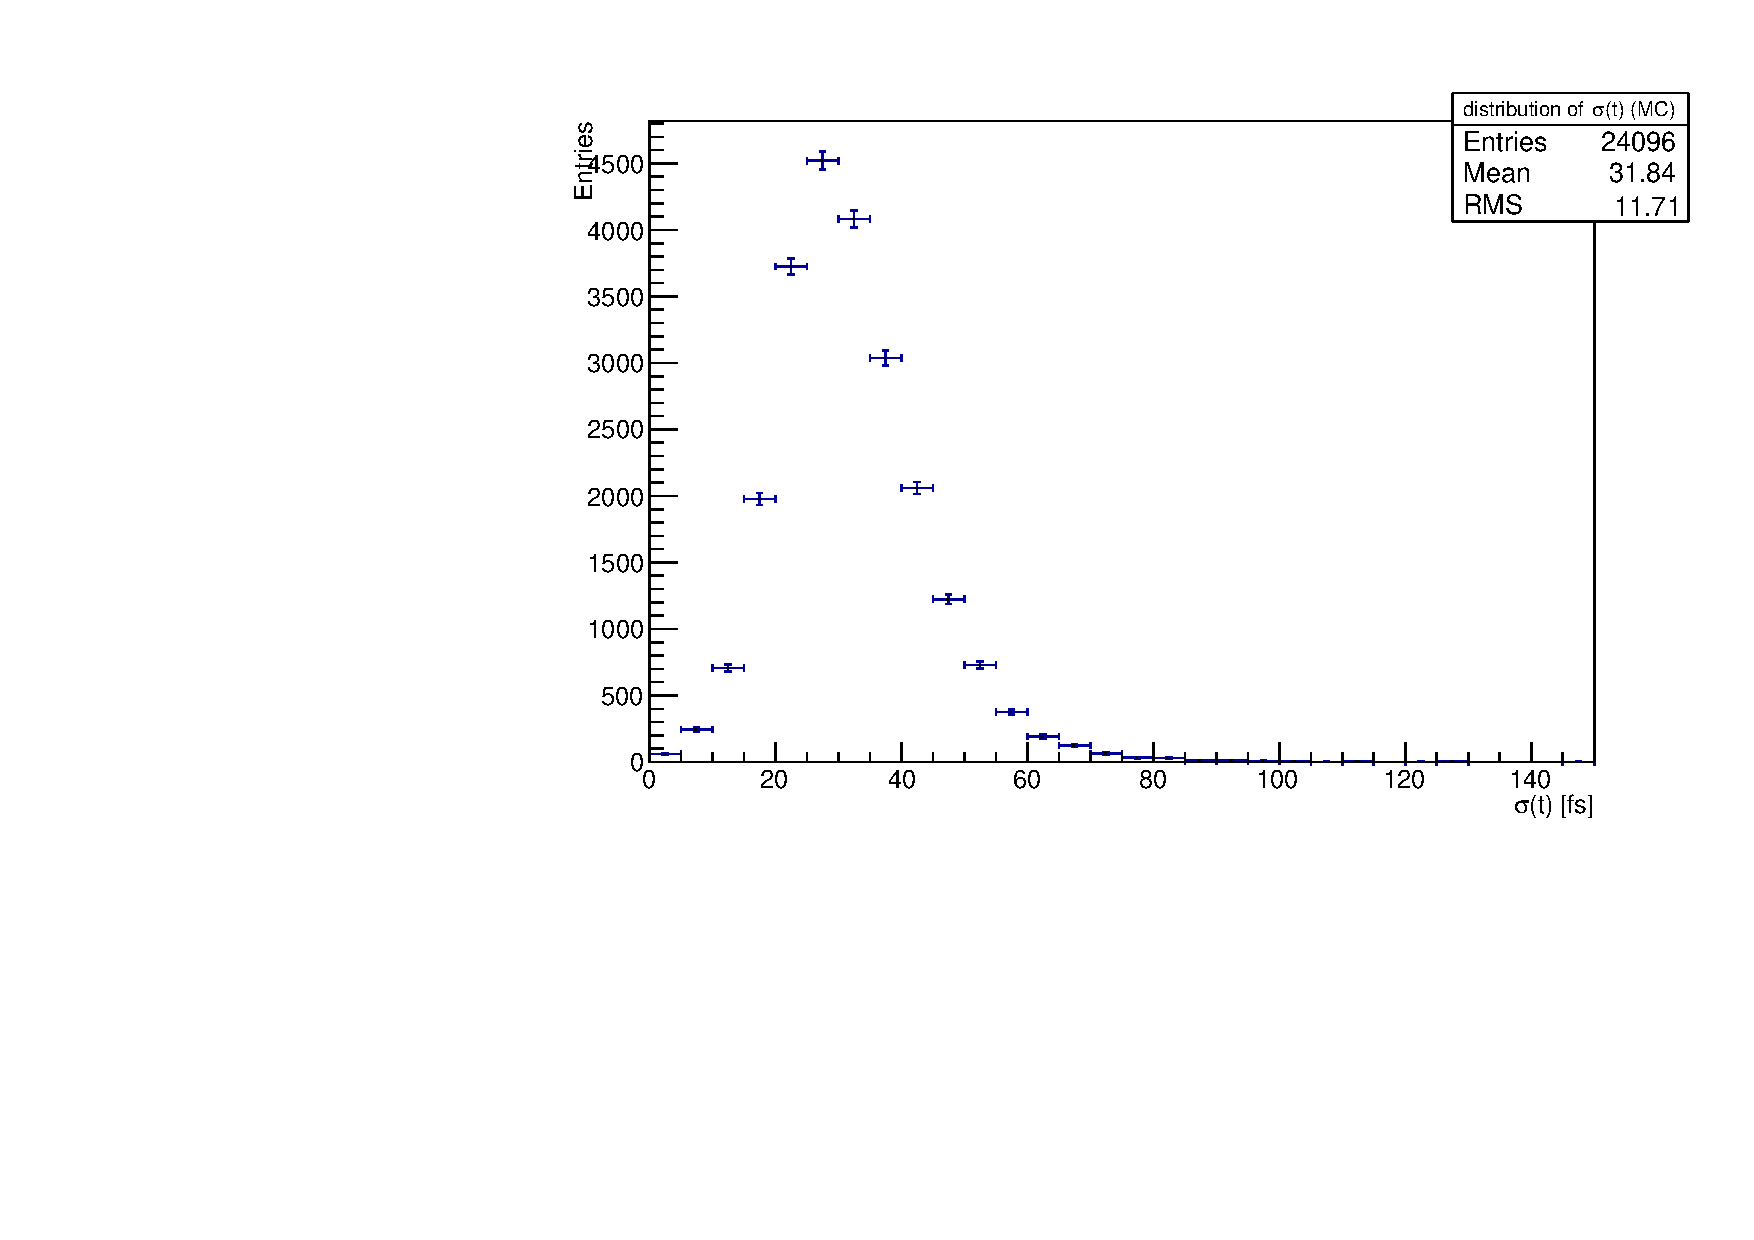
\includegraphics[width=5.5cm,height=4.7cm]{plots/Bs_cterr_MC.pdf}
\end{figure}

\column{.55\textwidth}

Fit double Gaussian to distribution of $\Delta t = t_{true} - t_{observed}$ in every Bin, on MC \newline

Derive effective resolution from Dilution of CP-observables 

\end{columns}

\end{frame}

\begin{frame}
\frametitle{Resolution}


\begin{figure}
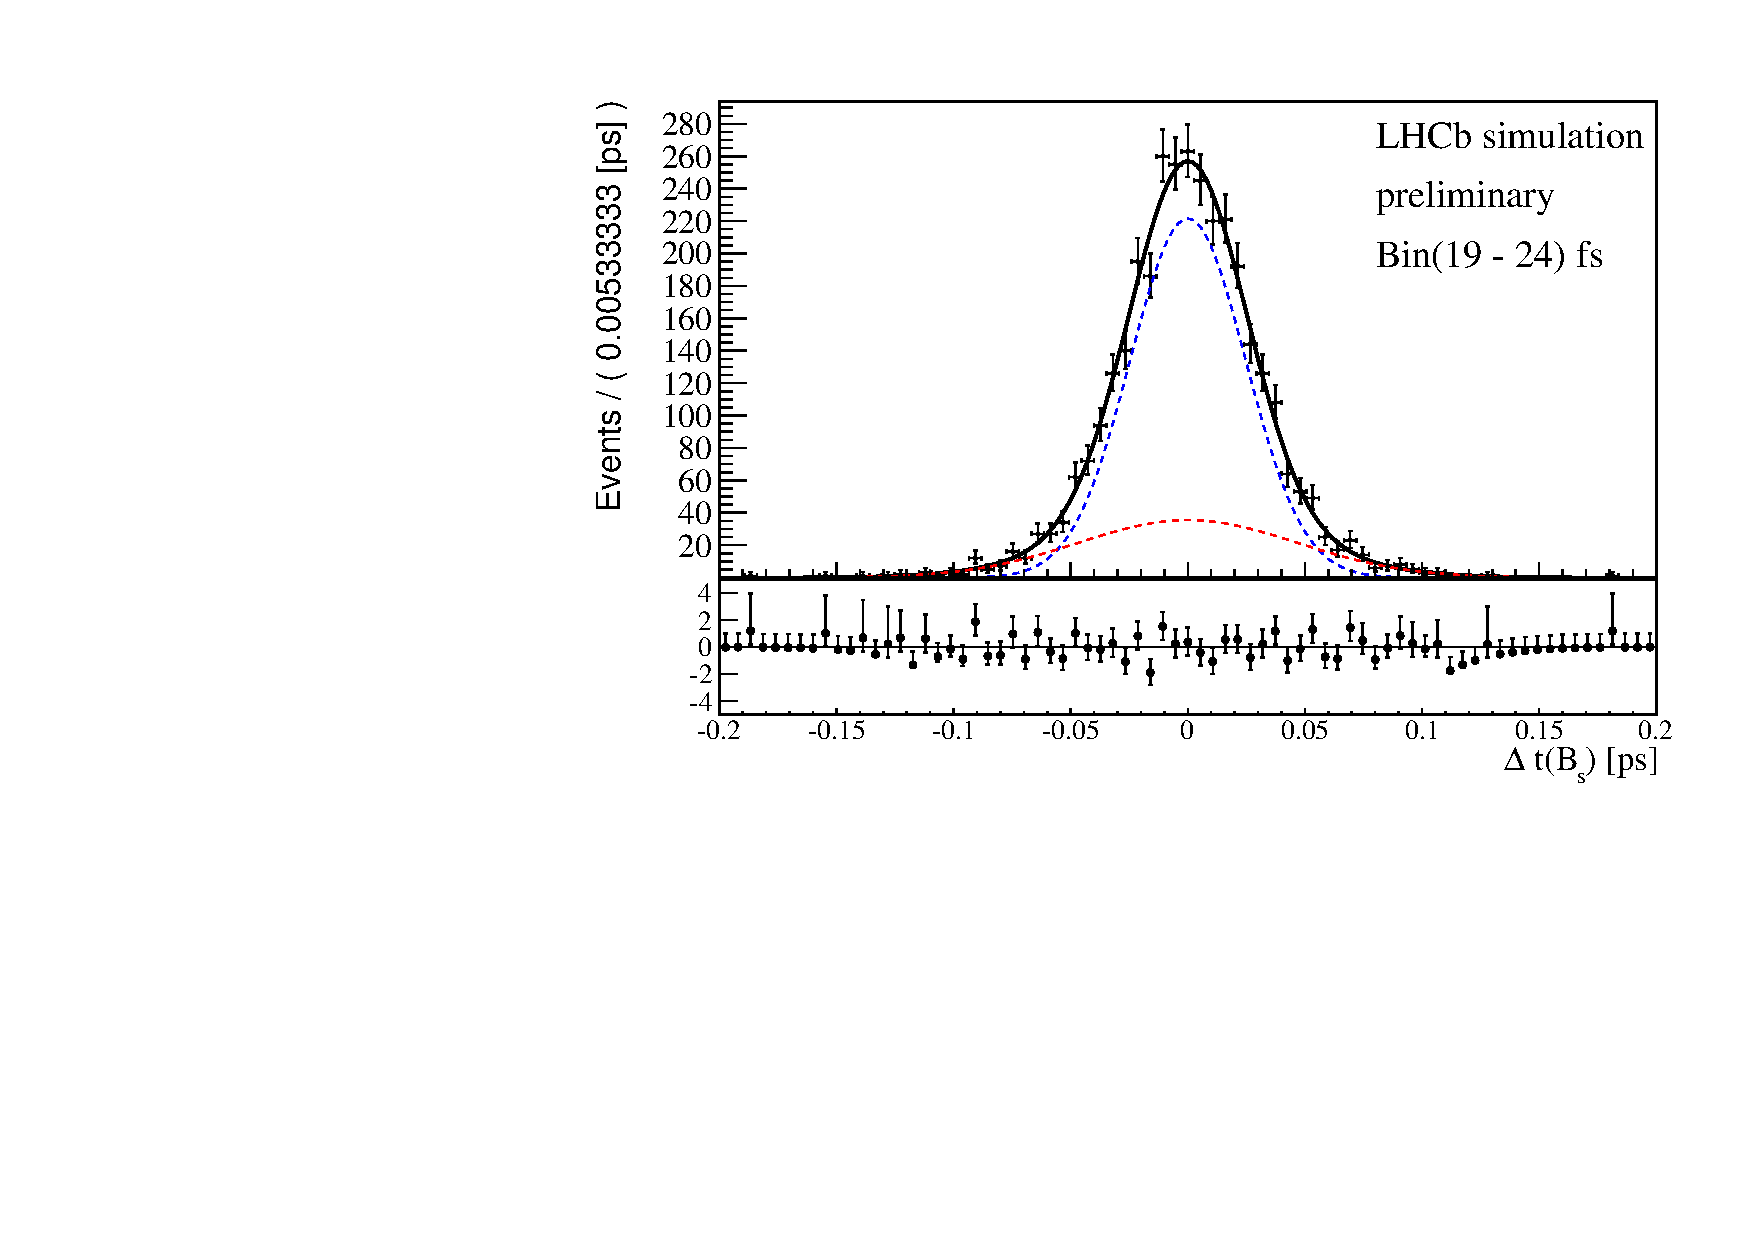
\includegraphics[width=6.0cm,height=4.7cm]{plots/SignalMC_19to24.pdf}
\end{figure}

\[\mathcal{D} = f_{1}e^{-\sigma_{1}^{2}\Delta m_{s}^{2}/2} + (1-f_{1})e^{-\sigma_{1}^{2}\Delta m_{s}^{2}/2}, \mathcal{D}\in [0,1]\] 

\[\sigma_{eff} = \sqrt{(-2/\Delta m_{s}^{2}) \ln{D}}\]

\end{frame}


\begin{frame}
\frametitle{Resolution}

Plot $\sigma_{t}$ from decay tree fitter against $\sigma_{eff}$ from Gaussian fits 

\begin{figure}
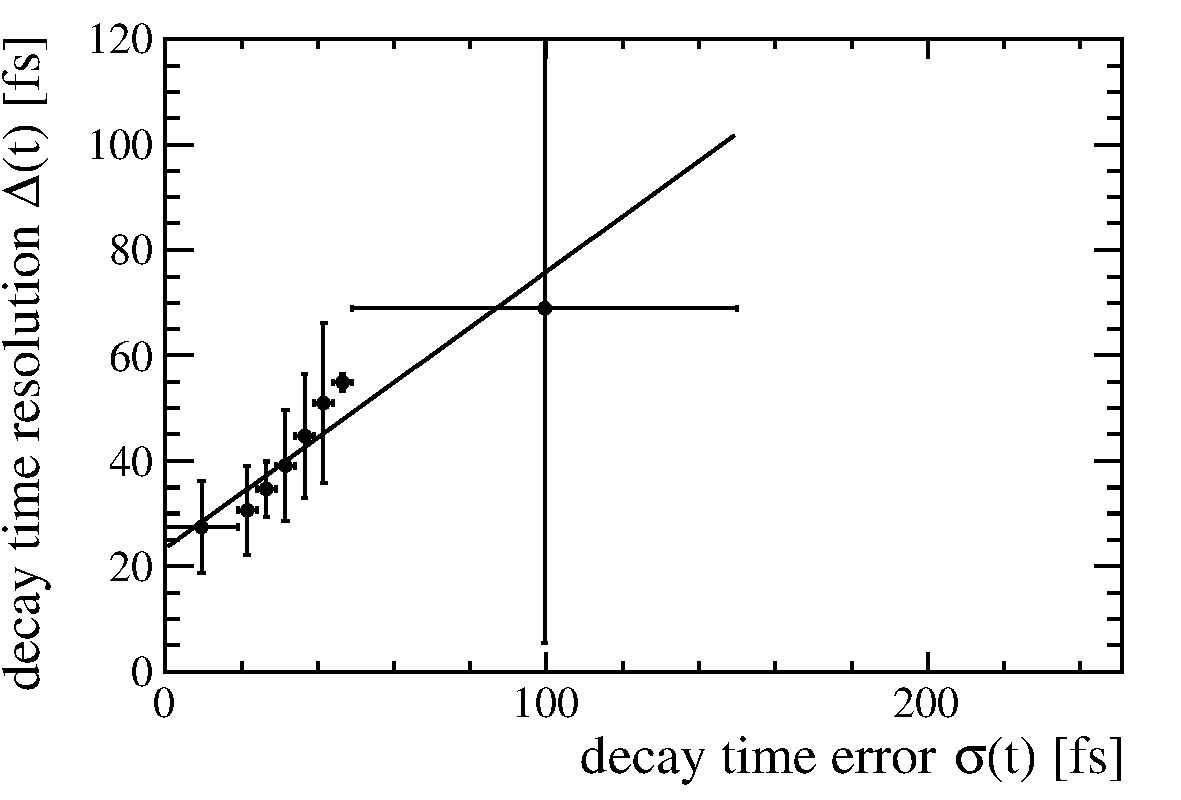
\includegraphics[width=6.0cm,height=4.7cm]{plots/ProperTimeReso_MC_onlyDsKpipi.pdf}
\end{figure}

Fitted with first order polynomial 

\end{frame}


\begin{frame}
\frametitle{Resolution}

\vspace{-1cm}

\begin{columns}

\column{.55\textwidth}

\begin{figure}
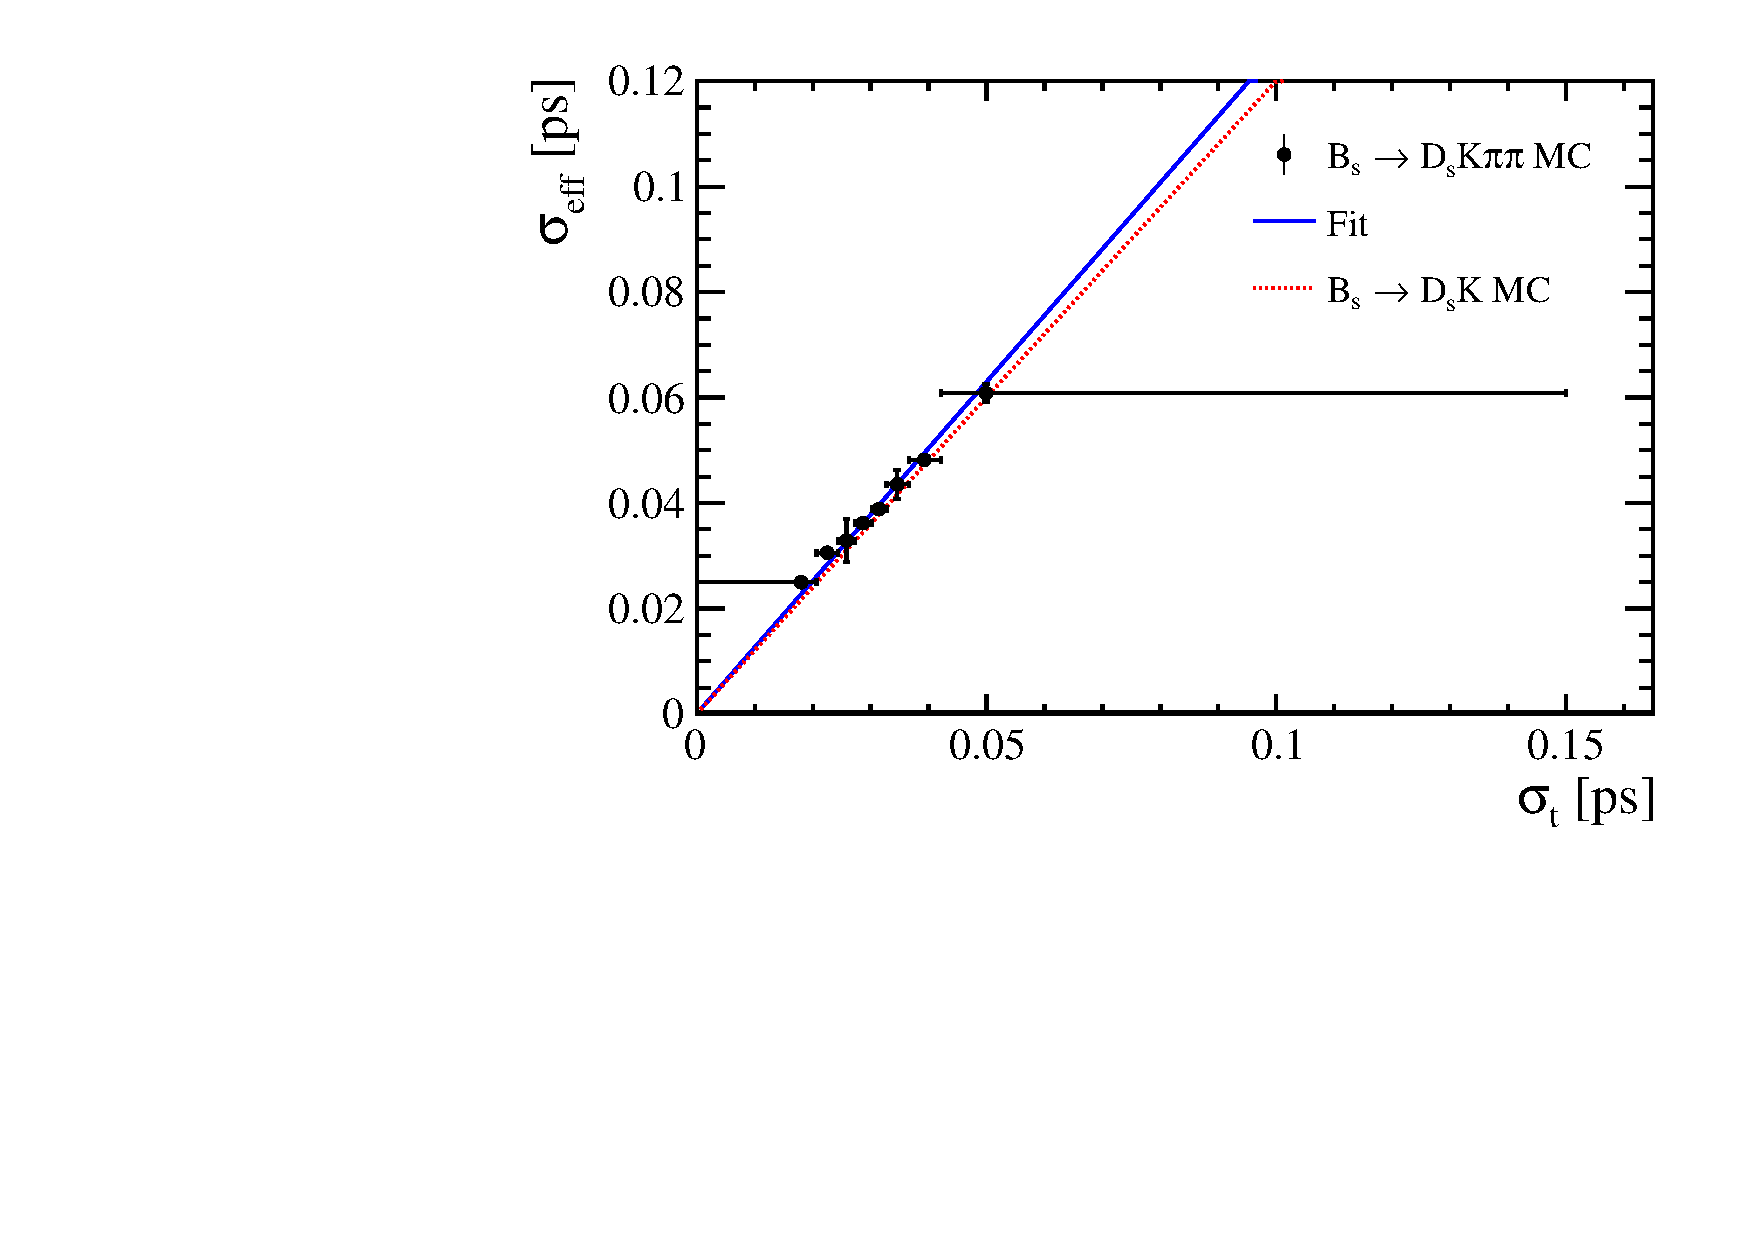
\includegraphics[width=6.0cm,height=4.7cm]{plots/ProperTimeReso_MC.pdf}
\end{figure}


\column{.55\textwidth}


comparison of \newline  
\textcolor{black}{$B_{s}\to D_{s}K\pi\pi$,MC} \newline
 \textcolor{blue}{$B_{s}\to D_{s}K$,MC} \newline
 \textcolor{red}{$B_{s}\to D_{s}K$,Data}



\end{columns}

$\rightarrow$ assume $\frac{\sigma_{eff}(\sigma_{t})_{D_{s}K,Data}}{\sigma_{eff}(\sigma_{t})_{D_{s}K,MC}} \approx \frac{\sigma_{eff}(\sigma_{t})_{D_{s}K\pi\pi,Data}}{\sigma_{eff}(\sigma_{t})_{D_{s}K\pi\pi,MC}}$ \newline

$\Leftrightarrow$ $\sigma_{eff}(\sigma_{t})_{D_{s}K\pi\pi,Data} \approx \frac{\sigma_{eff}(\sigma_{t})_{D_{s}K,Data}}{\sigma_{eff}(\sigma_{t})_{D_{s}K,MC}} \cdot \sigma_{eff}(\sigma_{t})_{D_{s}K\pi\pi,MC}$

\bigskip

\bfseries

Might be able to get LTU data by re-stripping due to HLT bug !

\normalfont

\end{frame}


\begin{frame}

\Huge \bfseries


\begin{center}

TD-Amplitude Fit using MINT

\end{center}

\normalsize
\normalfont

\end{frame}



\begin{frame}[plain]
%	\frametitle{TD Amplitude Analysis}

	\centering
	\vspace{-1cm}
		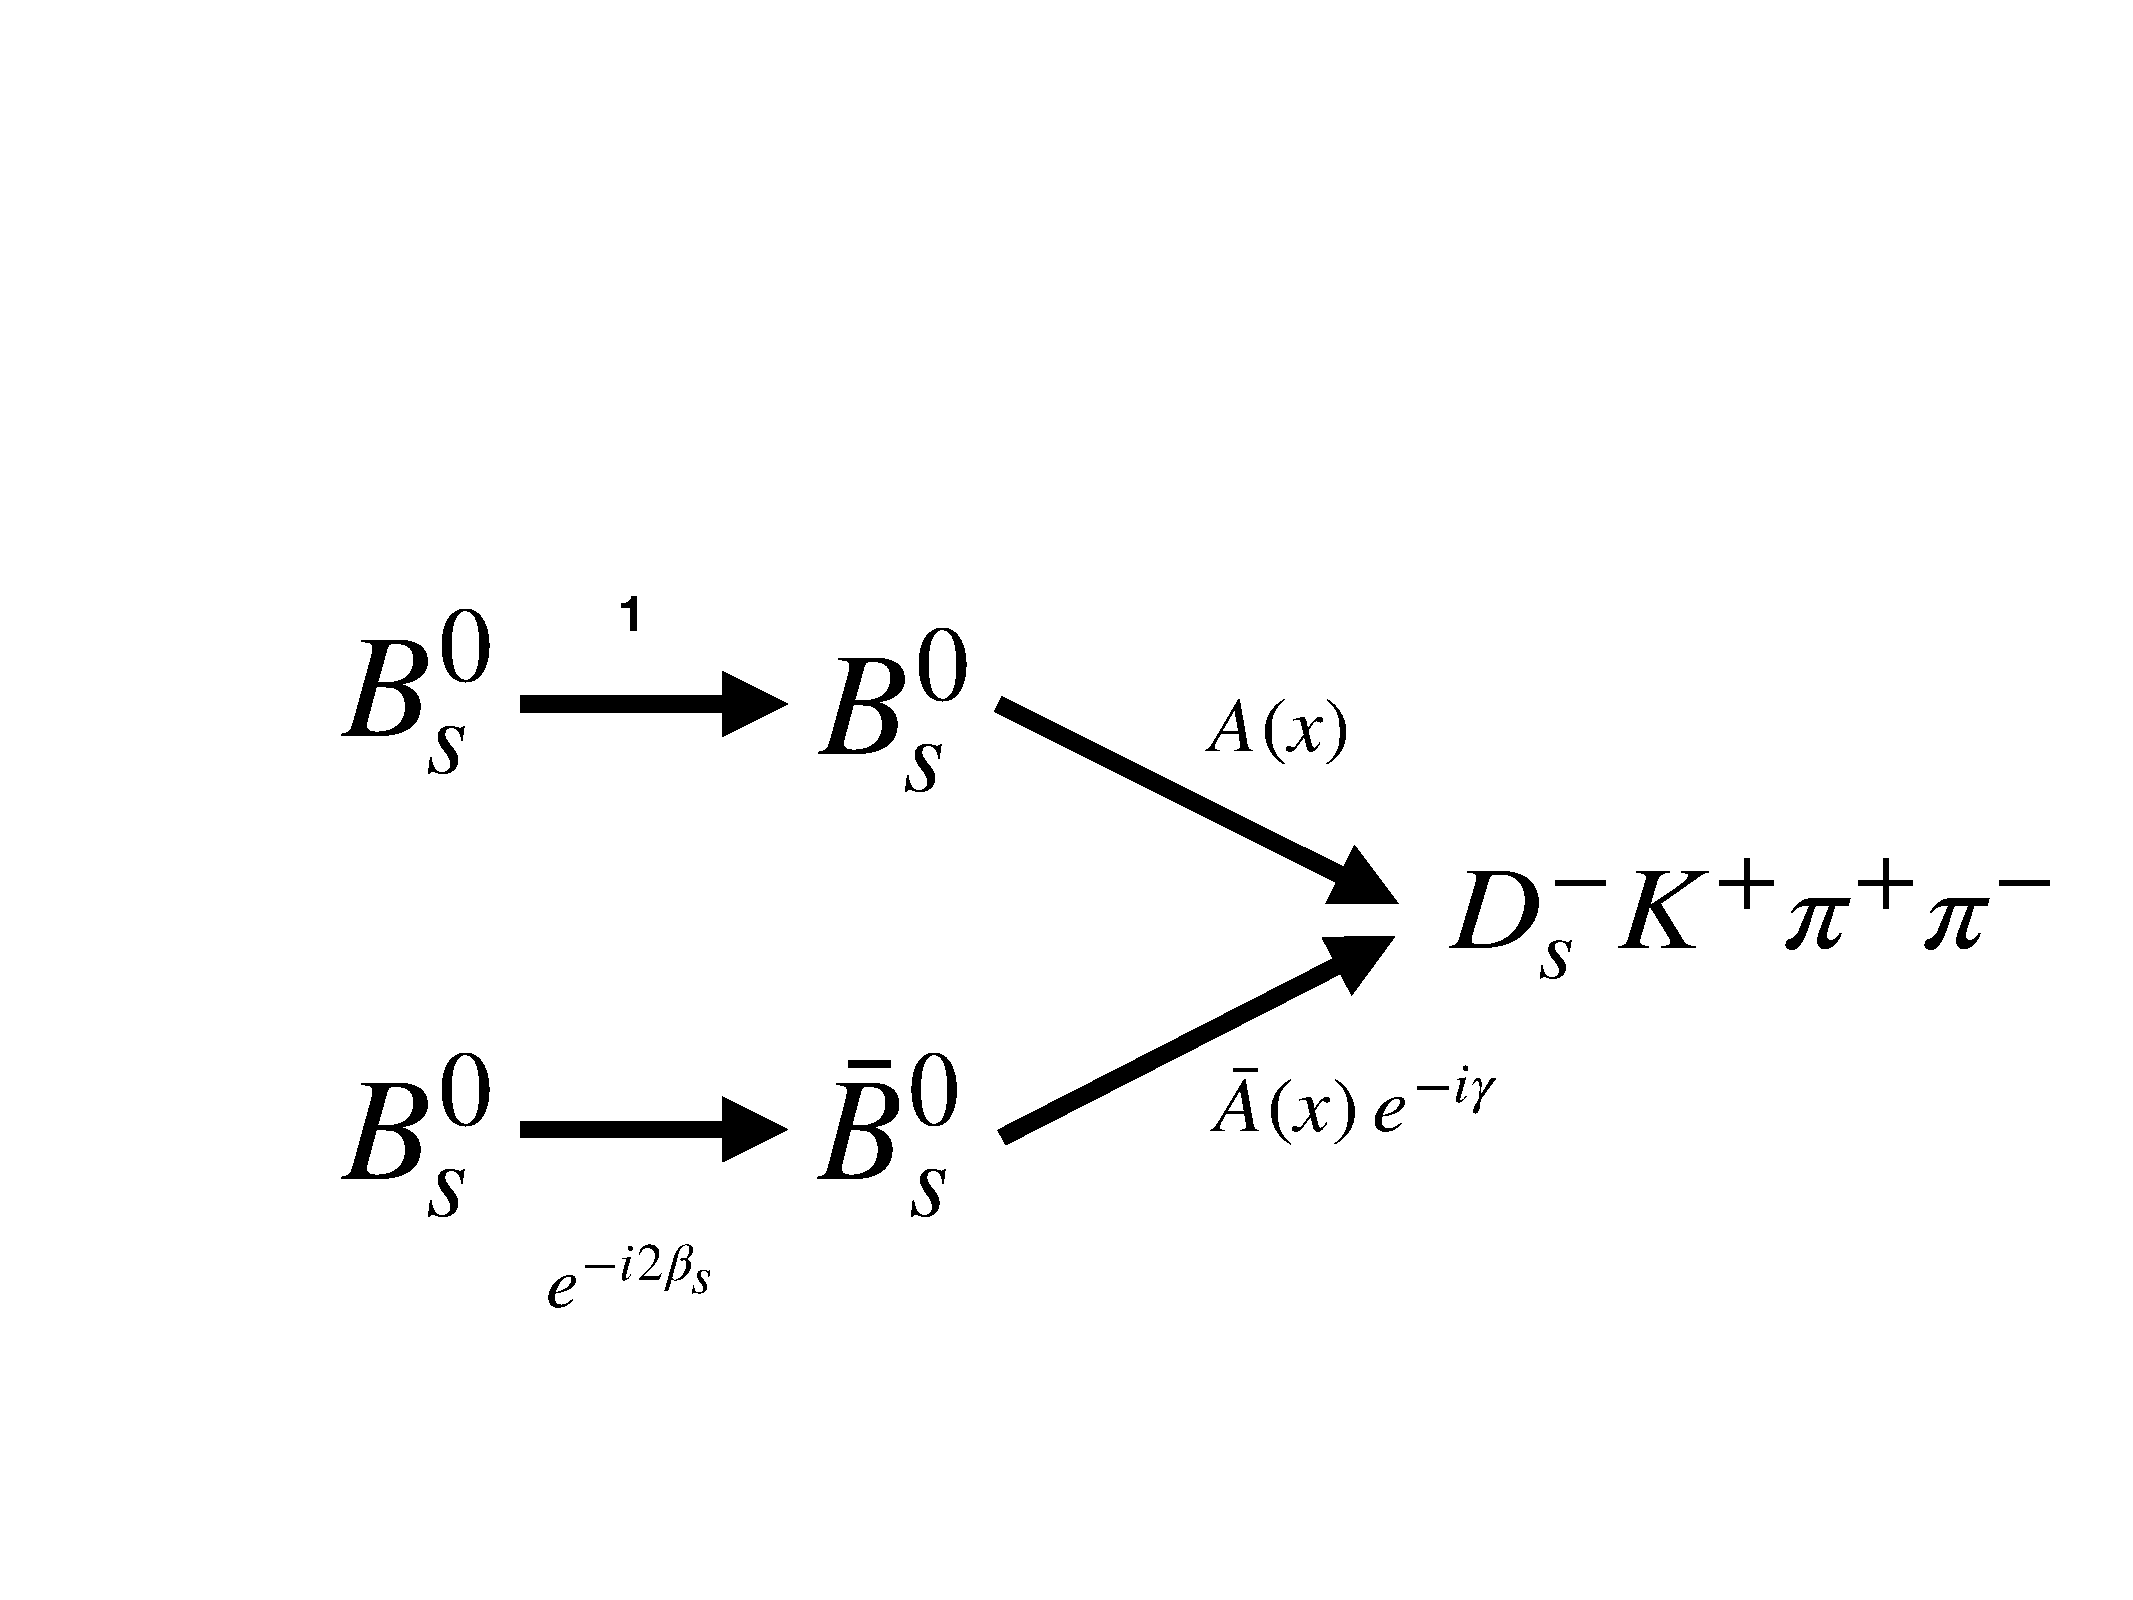
\includegraphics[width=0.49\textwidth, height = !]{plots/Bs_gamma.pdf} 	
		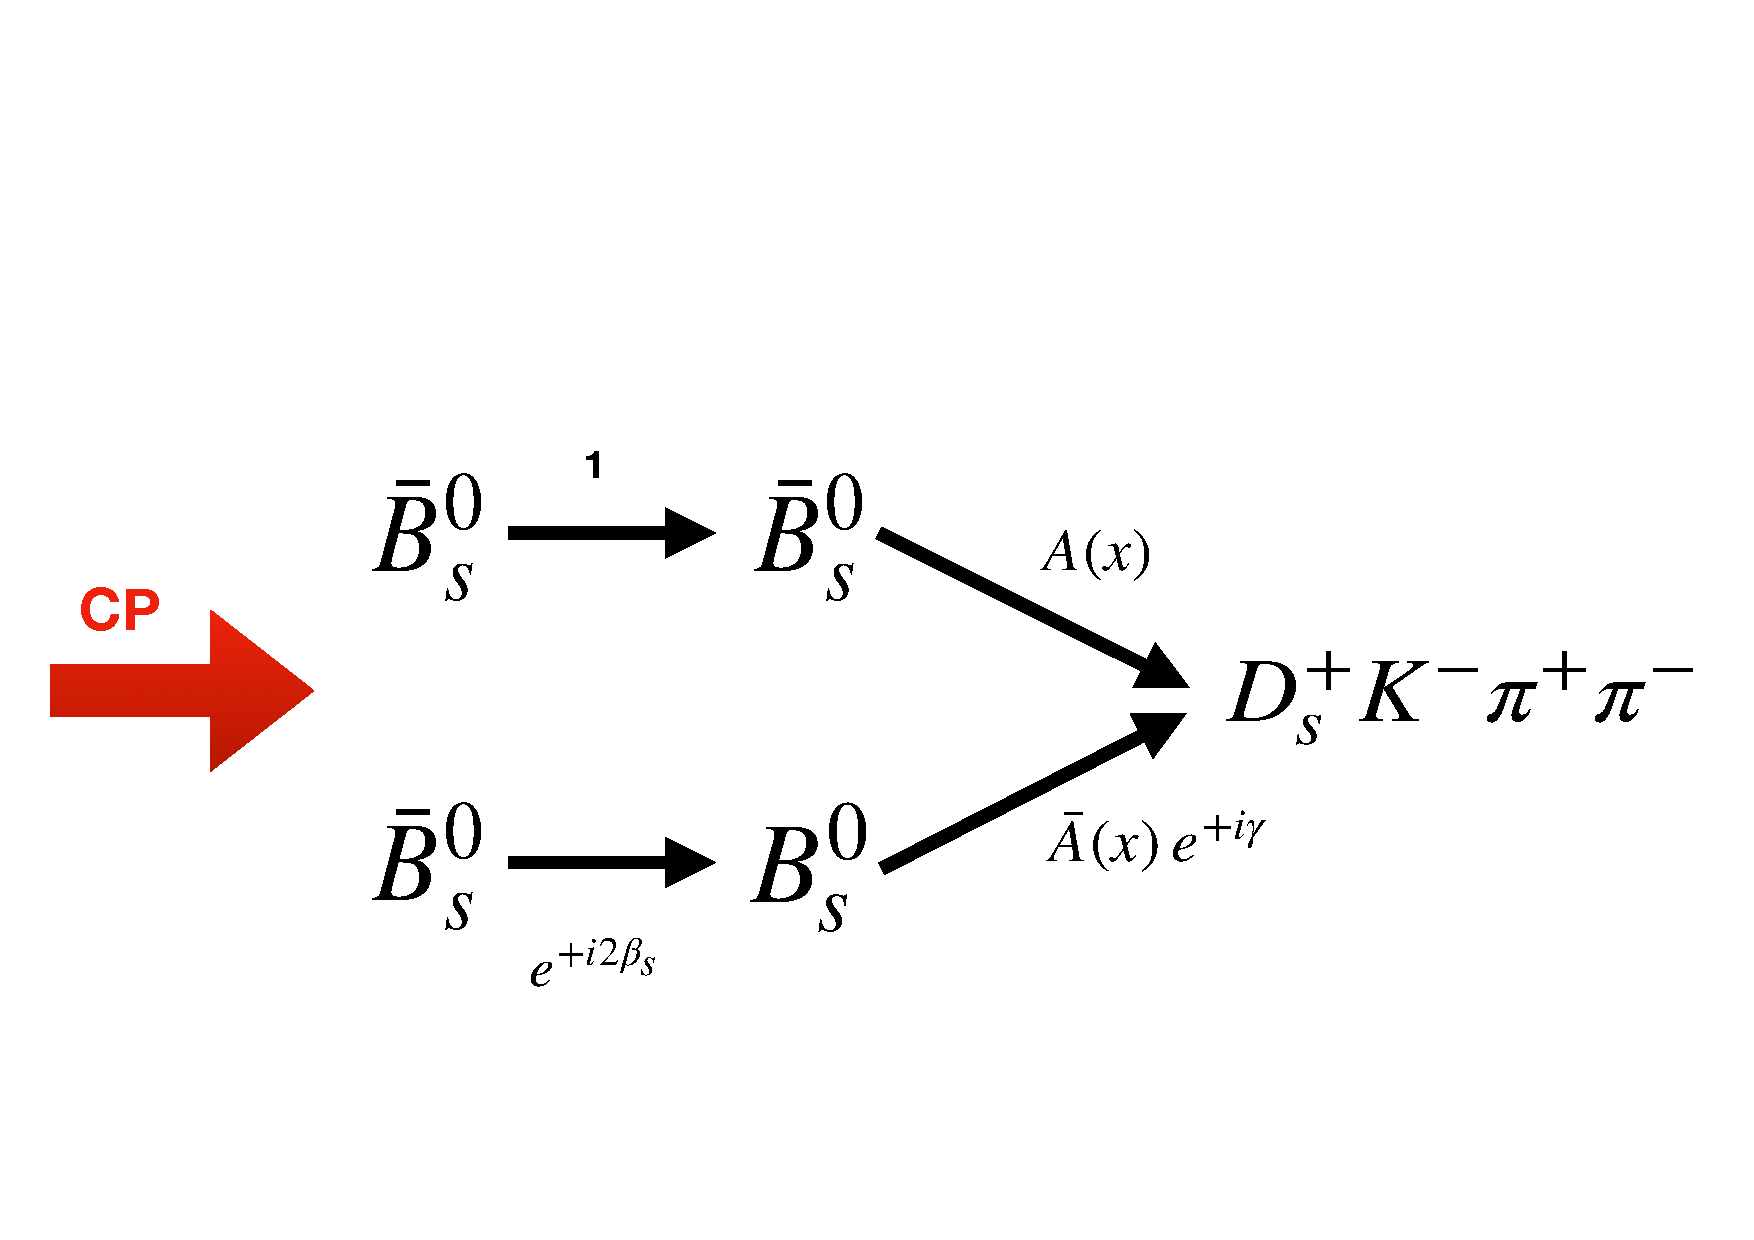
\includegraphics[width=0.49\textwidth, height = !]{plots/Bs_gamma_CP.pdf} 	
		
		
	\small
		\textbf{Full time-dependent amplitude PDF:}
		\scriptsize
	\begin{block}{}
\begin{align*}
	P(x,t,q_t,q_f) &\propto  [
	 \left( \vert A(x) \vert^2 + \vert \bar A(x) \vert^2 \right) \, \text{cosh} \left( \frac{\Delta \Gamma \, t}{2}\right) \\
	 & + q_t q_f \left( \vert A(x) \vert^2 - \vert \bar A(x) \vert^2 \right) \, \text{cos} \left( \Delta m_s \, t \right)  \\
	 & -2 \text{Re}\left( A(x)^{*}  \bar A(x) \, e^{-i q_f (\textcolor{red}{\gamma - 2\beta_s})}  \right) \, \text{sinh} \left( \frac{\Delta \Gamma \, t}{2}\right)  \\
	 & -2 q_t q_f \text{Im}\left( A(x)^{*}  \bar A(x) \, e^{-i q_f (\textcolor{red}{\gamma - 2\beta_s})}  \right)\, \text{sin} \left( \Delta  m_s \, t \right)  ]  e^{- \Gamma t}
\end{align*}
	\end{block}
%\newline
%\\

%	\small
$q_t = +1,0,-1$ for a $B_s^{0}$, no-,  ($\bar B_s^{0}$) tag  \\ 
$q_f$ = +1 $ $(-1) for $D_s^{-} K^{+} \pi\pi$ ($D_s^{+} K^{-} \pi\pi$) final states. 
				
\end{frame}





\begin{frame}
	\frametitle{Amplitude Analysis}

	\centering
	\small
	\textbf{Phasespace-integrated PDF:}
	\scriptsize
%Integrating over the phasespace, we get
	\begin{block}{}
\begin{align*}
	\int P(x,t,q_t,q_f) \text d x &\propto   [
	\, \text{cosh} \left( \frac{\Delta \Gamma \, t}{2}\right) \\
	 & + q_t q_f \left( \frac{1-r^2}{1+r^2} \right) \, \text{cos} \left( m_s \, t \right)  \\
	 & -2 \left( \frac{\kappa \, r \, \text{cos}(\delta - q_f(\gamma - 2 \beta_s))}{1+r^2}  \right) \, \text{sinh} \left( \frac{\Delta \Gamma \, t}{2}\right)  \\
	 & -2 q_t q_f \left( \frac{\kappa \, r \, \text{sin}(\delta - q_f(\gamma - 2 \beta_s))}{1+r^2}   \right)\, \text{sin} \left( m_s \, t \right)  ]  e^{- \Gamma t} \\
	 &=   [
	\, \text{cosh} \left( \frac{\Delta \Gamma \, t}{2}\right) 
	  + q_t q_f \, \textbf{C} \, \text{cos} \left( m_s \, t \right)   \\
	  & - \textcolor{red}{\kappa} \, \textbf{D}_{q_f} \, \text{sinh} \left( \frac{\Delta \Gamma \, t}{2}\right)  
	  - q_t \, \textcolor{red}{\kappa} \, \textbf{S}_{q_f}\, \text{sin} \left( m_s \, t \right)  ]  e^{- \Gamma t}
\end{align*}
	\end{block}
%where the $C,D_{q_f},S_{q_f}$ are defined exactly as for $D_s K$.
%The coherence factor is defined as :
%\begin{align*}
\vspace{0.2cm}
\small
$r \equiv \, \frac{\sqrt{\int \vert \bar A(x) \vert^2\text d x }}{\sqrt{\int \vert A(x) \vert^2\text d x}} $, 
$	\kappa \, e^{i\delta} \equiv \, \frac{\int A(x)^{*}  \bar A(x)  \text d x}{\sqrt{\int \vert A(x) \vert^2\text d x} \sqrt{\int \vert \bar A(x) \vert^2\text d x}  }$ %\end{align*}

\end{frame}



\begin{frame}
	\frametitle{Amplitude Analysis}

	\centering
		\small
	\textbf{Time-integrated, flavor averaged PDF:}
	
		\scriptsize

\begin{block}{}
\begin{align*}
	\int P(x,t,q_t,q_f) \, \text d t \, \text d q_t \, \text d q_f &\propto   \left( \vert A(x) \vert^2 + \vert \bar A(x) \vert^2 \right) \equiv \vert A^{eff}(x) \vert^2
\end{align*}
\end{block}

	\begin{block}{}
	\begin{itemize}
		\item No sensitivity to $\gamma$
		\item Useful to identify contributing amplitude components
	\end{itemize}
	\end{block}	

\end{frame}



\begin{frame}
\frametitle{TD-MINT}

\begin{itemize}

\item We implemented time-dependence + acceptance + resolution into MINT 

\item Now want to generate toys and validate the fitter

\item First, take time-integrated MINT to fit contributing amplitude components

\item Use fitted amplitudes to generate toys with TD-MINT

\item Fit toys, examine results and compare phasespace-integrated to full fit 

\item additional tests of acceptance + resolution implementation possible, by comparing results to B2DX fitter package 

\end{itemize}


\end{frame}


\begin{frame}
	\frametitle{Time integrated amplitude fit}

	\centering
	
	\begin{figure}[hp]
	\centering
%		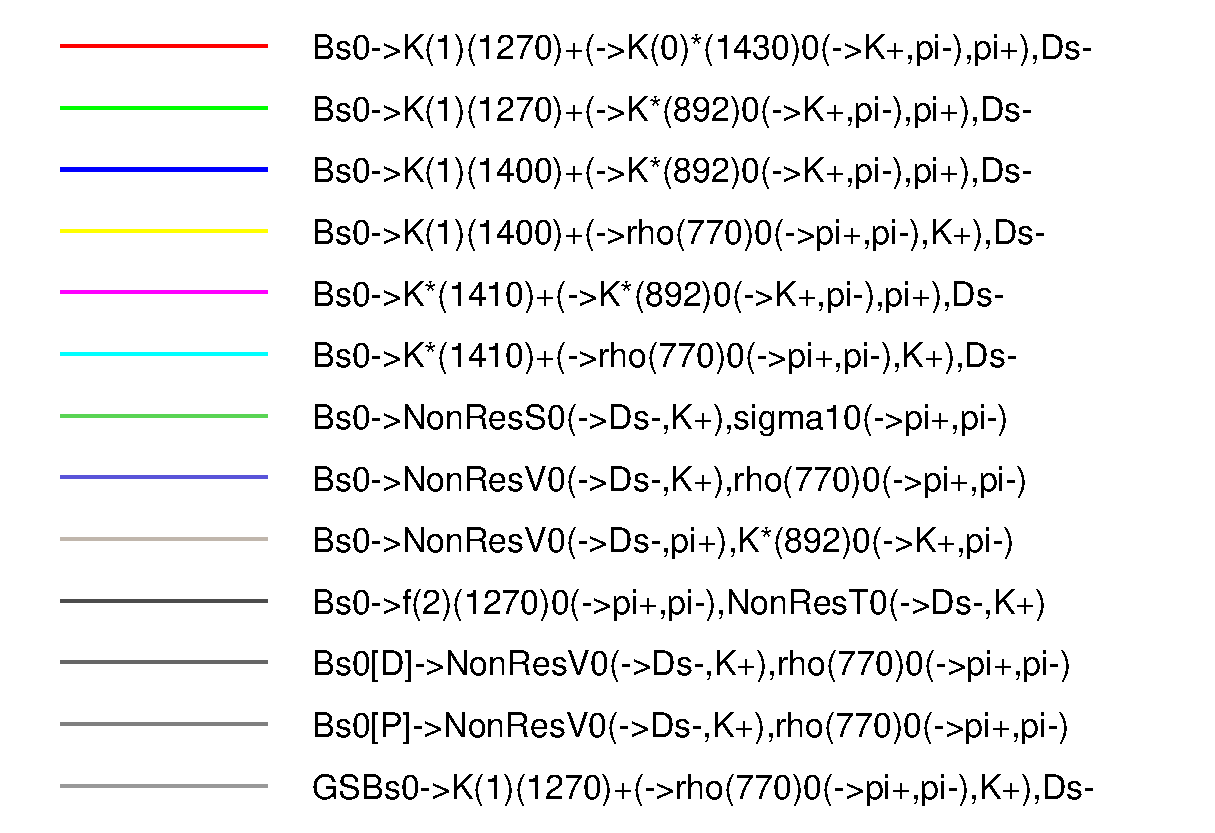
\includegraphics[width=0.35\textwidth, height = 3.cm]{plots/WithAmps__leg.eps} 
		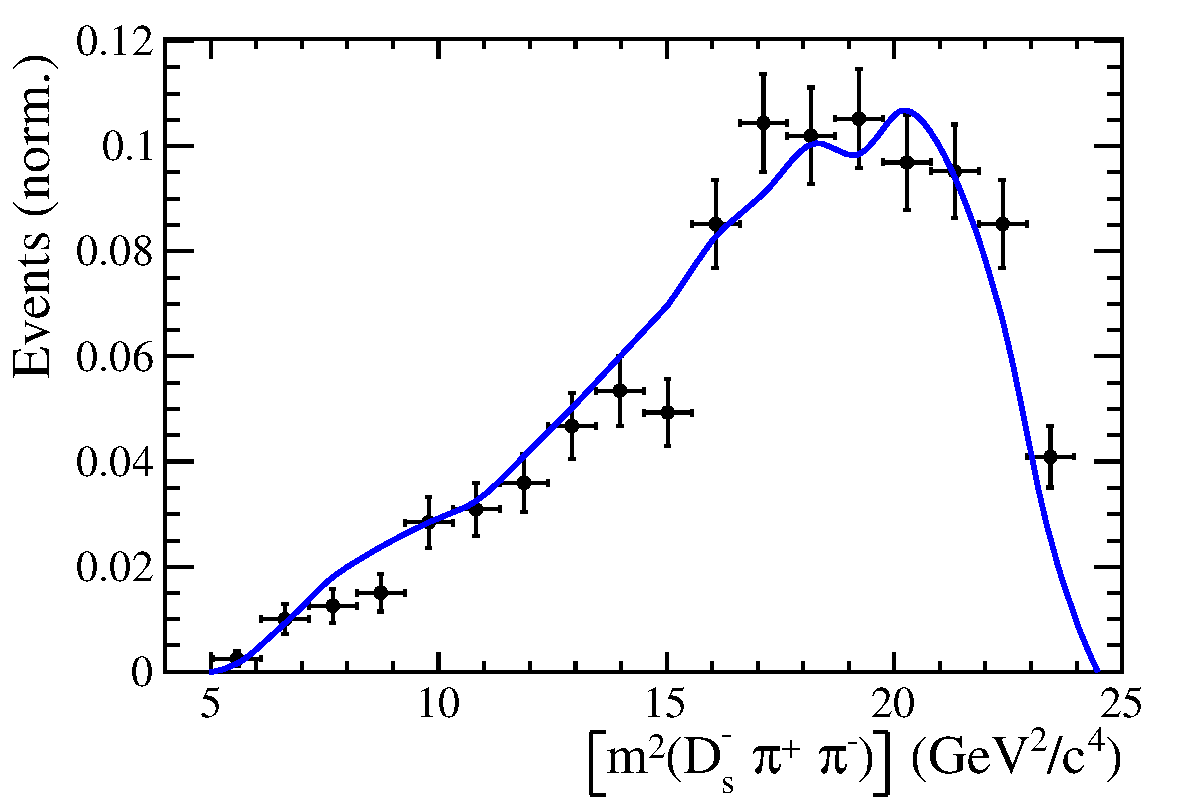
\includegraphics[width=0.35\textwidth, height = 3.cm]{plots/s_Dspipi.pdf} 
		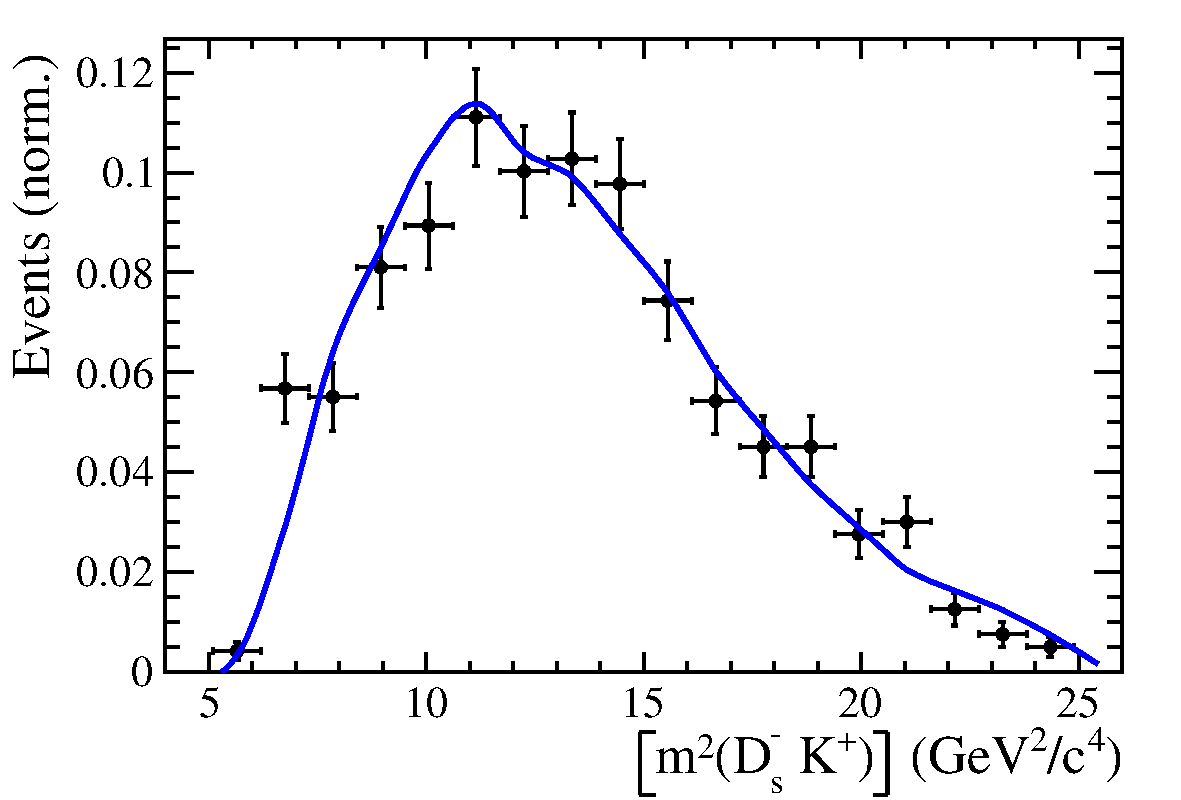
\includegraphics[width=0.35\textwidth, height = 3.cm]{plots/s_DsK.pdf} 

		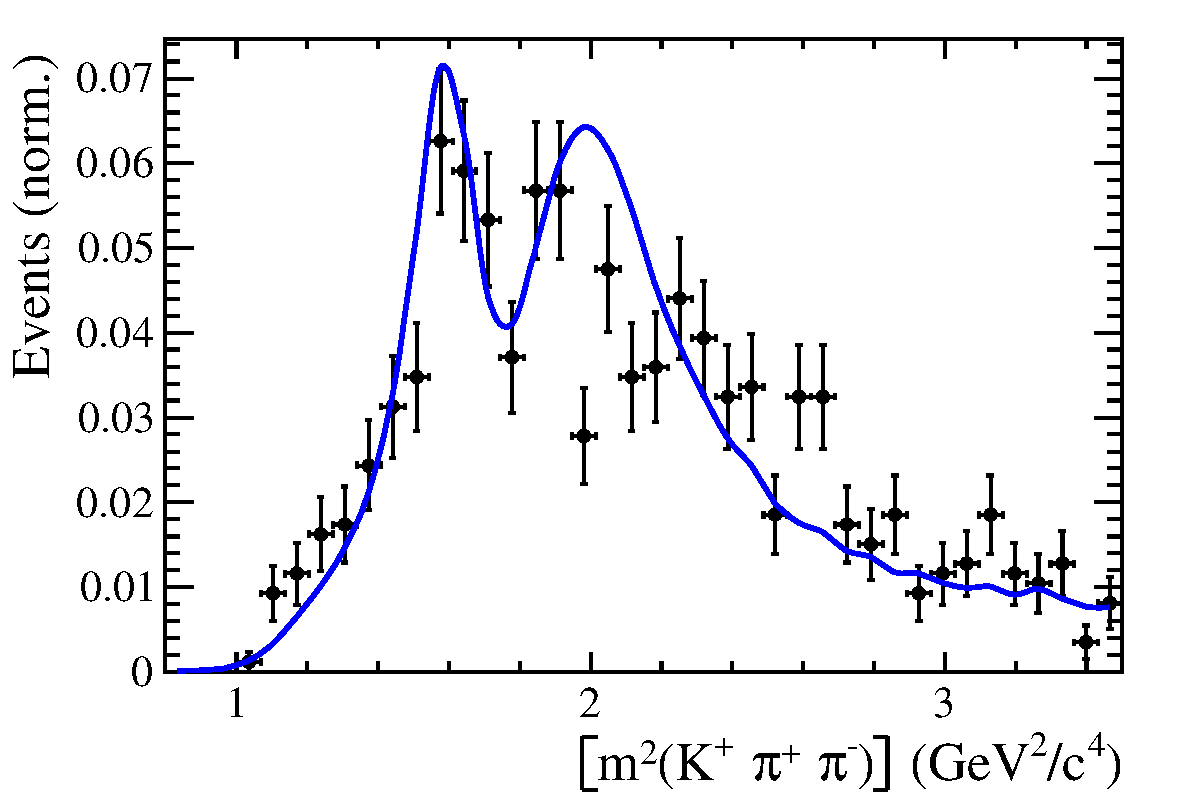
\includegraphics[width=0.35\textwidth, height = 3.cm]{plots/s_Kpipi.pdf} 
		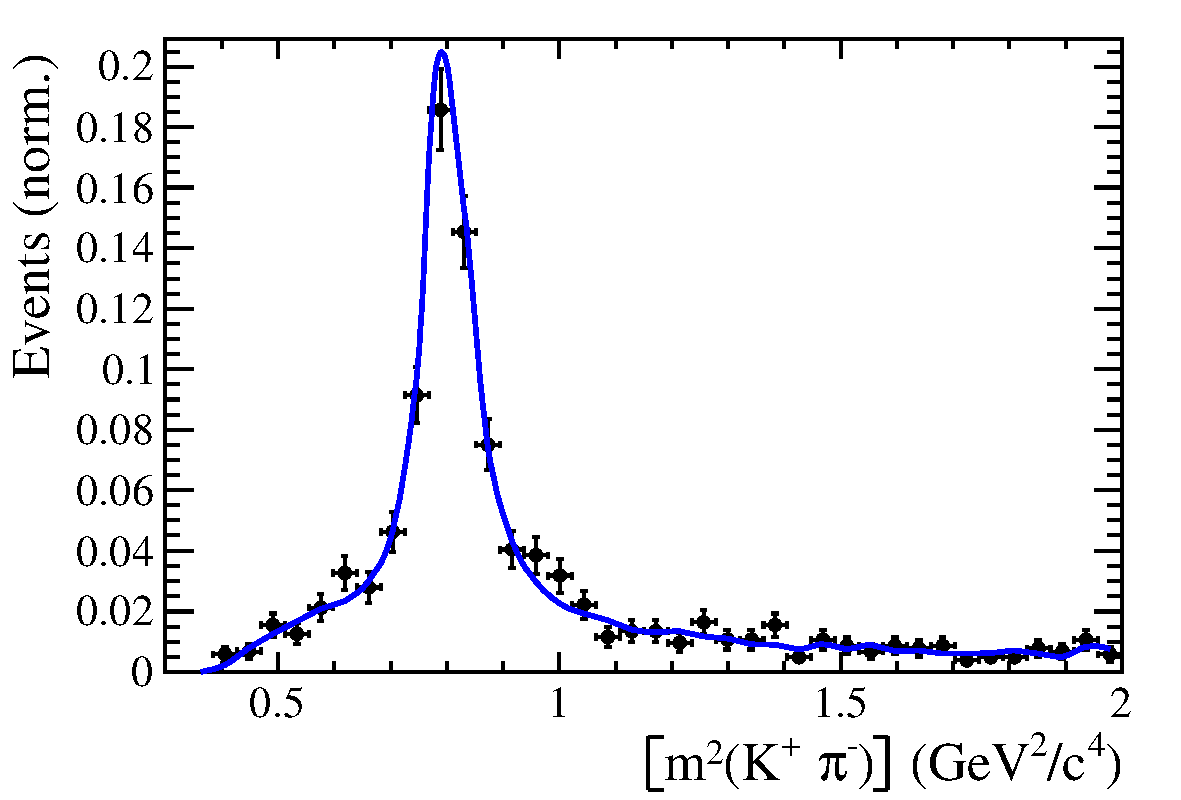
\includegraphics[width=0.35\textwidth, height = 3.cm]{plots/s_Kpi.pdf} 
		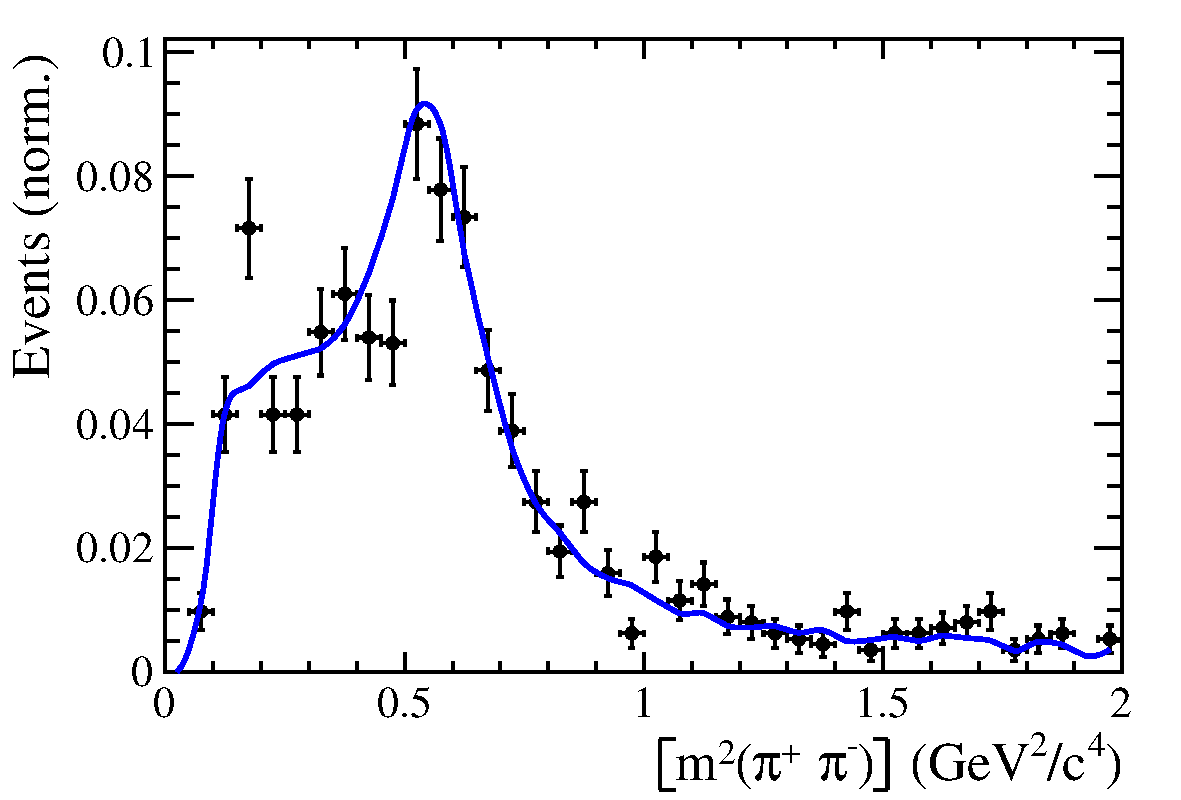
\includegraphics[width=0.35\textwidth, height = 3.cm]{plots/s_pipi.pdf} 		
	\end{figure}				
\end{frame}

\begin{frame}[fragile]
	\frametitle{Fit fractions}

	\centering
%      $F_i = \frac{\int ( \vert a_i  A_i(x) \vert^2 + \vert \bar a_i  \bar A_i(x) \vert^2 ) \, \text{d}x}{\int ( \vert A(x) \vert^2 + \vert\bar A(x) \vert^2 ) \, \text{d}x} $ \\
      $F^{eff}_i = \frac{\int  \vert a^{eff}_i  A^{eff}_i(x) \vert^2  \, \text{d}x}{\int  \vert A^{eff}(x) \vert^2 \, \text{d}x} $ \\


	\tiny
%	\centering
\begin{verbatim} 
	(1) Bs0->K(1)(1270)+(->K(0)*(1430)0(->K+,pi-),pi+),Ds- = 0.0520926 +/- 0.0145326
	(2) Bs0->K(1)(1270)+(->K*(892)0(->K+,pi-),pi+),Ds- = 0.090921 +/- 0.0214
	(3) Bs0->K(1)(1400)+(->K*(892)0(->K+,pi-),pi+),Ds- = 0.315657 +/- 0.0320033
	(4) Bs0->K*(1410)+(->K*(892)0(->K+,pi-),pi+),Ds- = 0.127998 +/- 0.0175661
	(5) Bs0->NonResS0(->Ds-,pi+),K*(892)0(->K+,pi-) = 0.0265594 +/- 0.0114541
	(6) Bs0[D]->NonResV0(->Ds-,pi+),K*(892)0(->K+,pi-) = 0.0108669 +/- 0.0069929
	(7) Bs0->NonResA0(->sigma10(->pi+,pi-),Ds-),K+ = 0.0715845 +/- 0.0247102
	(8) Bs0->NonResV0(->Ds-,K+),sigma10(->pi+,pi-) = 0.139525 +/- 0.0321404
	(9) Bs0->K(1)(1270)+(->rho(770)0(->pi+,pi-),K+),Ds- = 0.16488 +/- 0.0379784
	(10) Bs0->K(1)(1400)+(->rho(770)0(->pi+,pi-),K+),Ds- = 0.071005 +/- 0.0218139
	(11) Bs0->K*(1410)+(->rho(770)0(->pi+,pi-),K+),Ds- = 0.0766048 +/- 0.014699
	(12) Bs0->NonResA0(->rho(770)0(->pi+,pi-),Ds-),K+ = 0.0210193 +/- 0.0104696
	 sum = 1.16871 +/- 0.0595647(fit)
\end{verbatim}	
				
\end{frame}

\begin{frame}
	\frametitle{Time dependent amplitude fit}

	\centering
	
	\begin{block}{}
	\begin{itemize}
		\item  Now time-dependent MINT extension
		\item Generate toys with different values for $\kappa$ 
		\item Compare sensitivity to $\gamma$ fitting with \\ \textbf{full PDF} and with \textbf{phasespace-integrated PDF}
		\end{itemize}
	\end{block}		
		
	\begin{block}{Assumptions}
	\begin{itemize}	
		\item Use amplitudes from flavor-averaged, time-integrated fit
		\item $r = 0.4$ (ratio of CKM elements) 
		\item PDG values for: $\tau,\Delta m_s, \Delta \Gamma, \beta_s$
		\item $\epsilon(x,t) = const.$, including resolution and acceptance   
		\item $\epsilon_{Tag} = 0.66, <\omega> = 0.4 $   
		\item $N_{signal} = 3000$ (Run1+15/16 data)		 
	\end{itemize}
	\end{block}	
			

\end{frame}

\begin{frame}
	\frametitle{Example Toy-Fit: $B_s \to D_s K \pi \pi$}

	\centering
	
	\begin{figure}[hp]
	\centering
		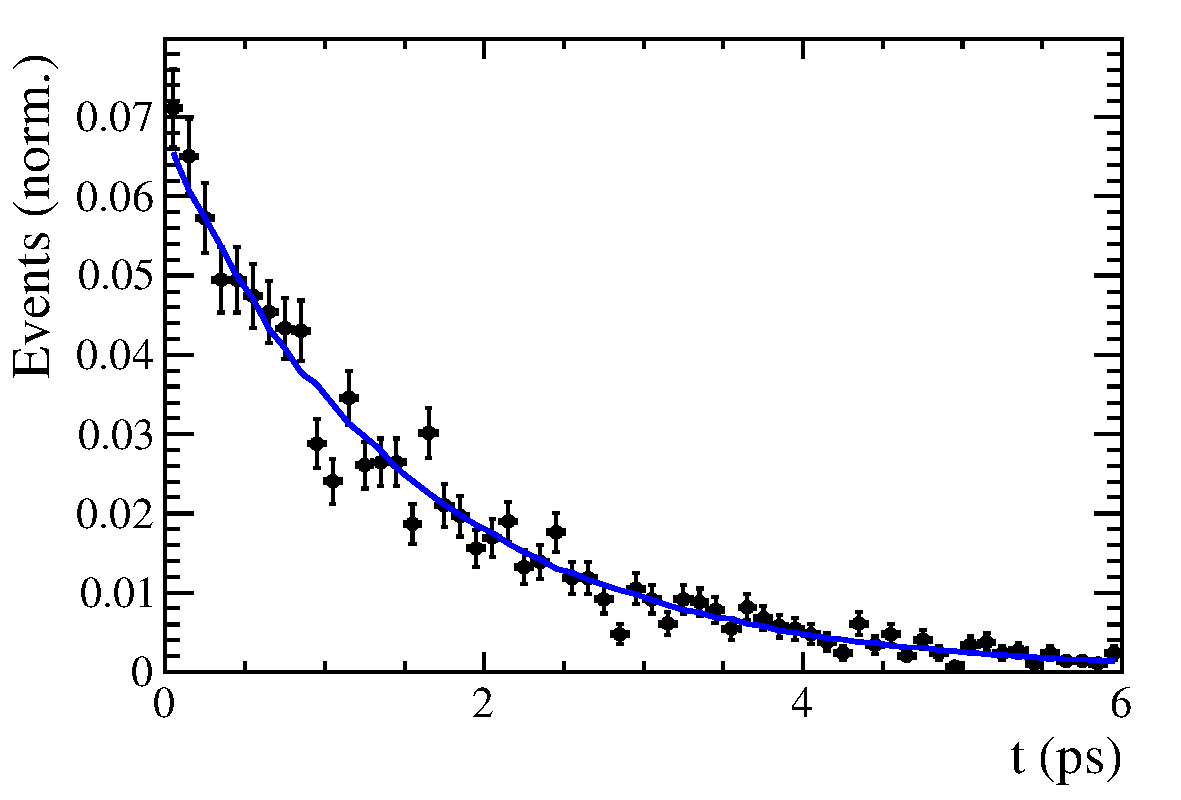
\includegraphics[width=0.35\textwidth, height = 3.cm]{plots_toys/h_t-eps-converted-to.pdf} 
		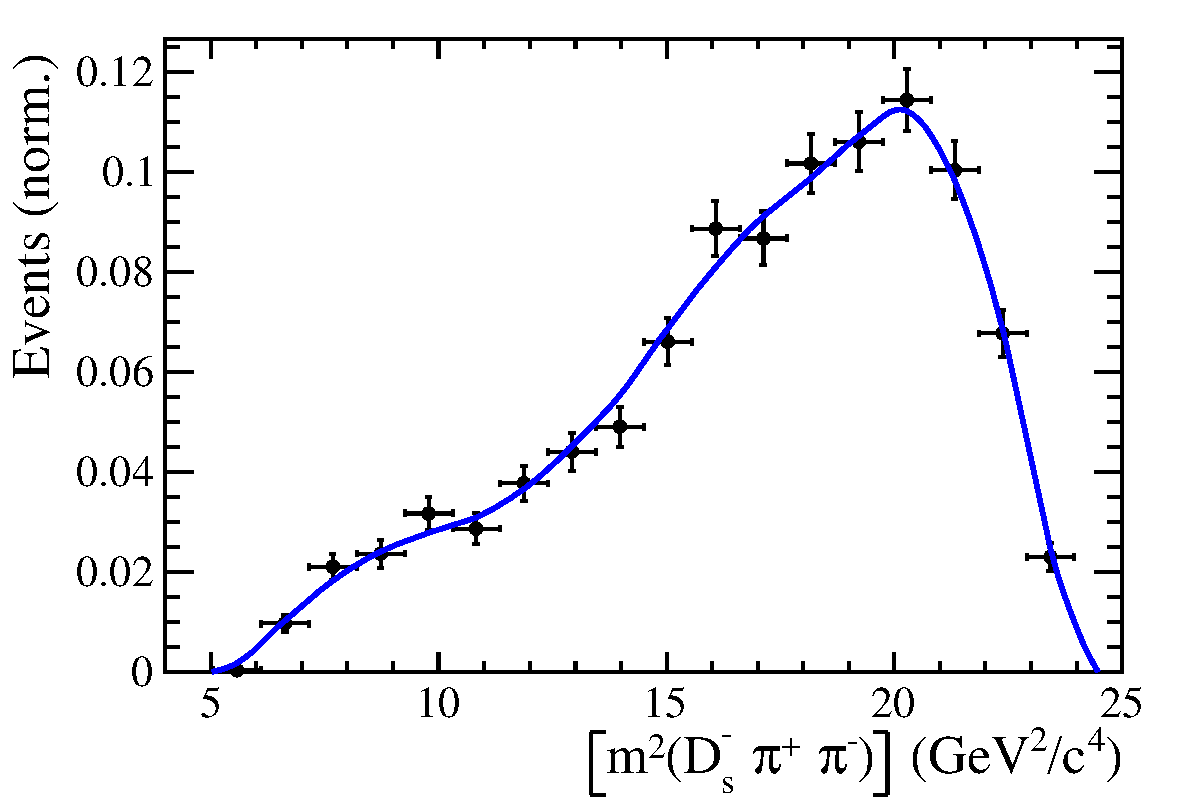
\includegraphics[width=0.35\textwidth, height = 3.cm]{plots_toys/s_Dspipi-eps-converted-to.pdf} 
		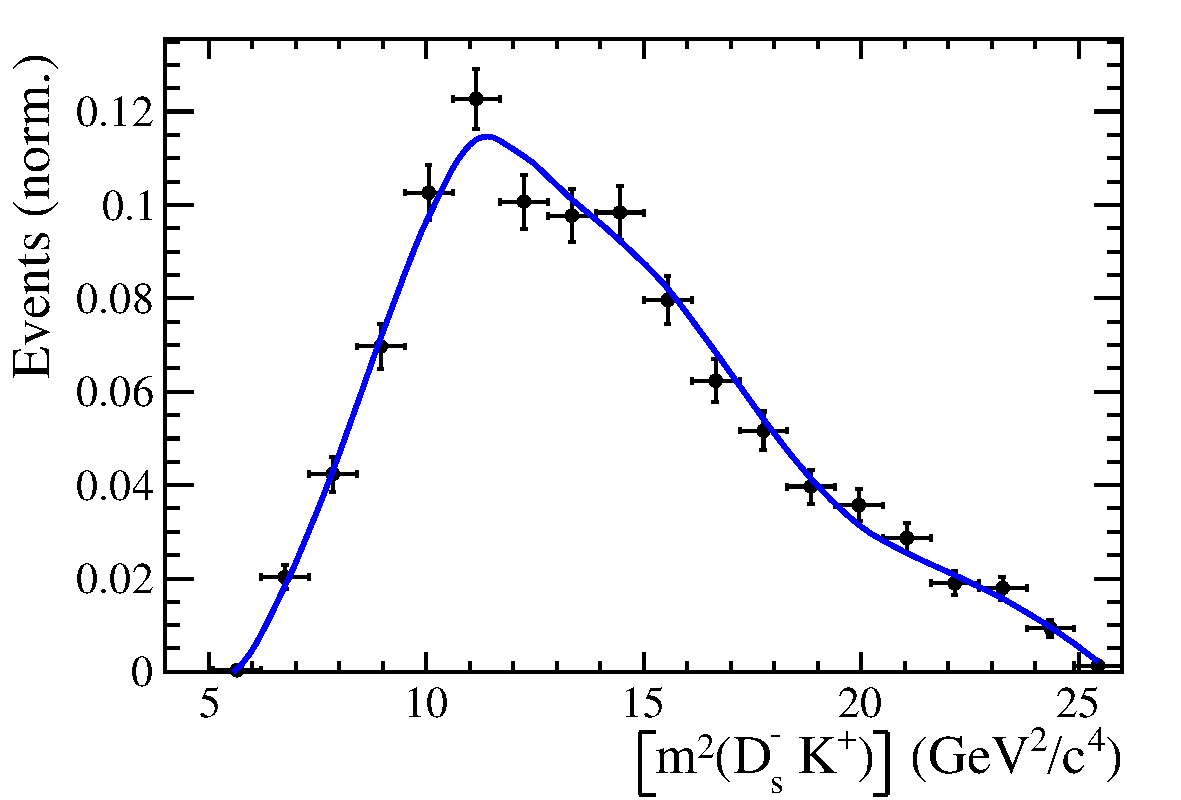
\includegraphics[width=0.35\textwidth, height = 3.cm]{plots_toys/s_DsK-eps-converted-to.pdf} 

		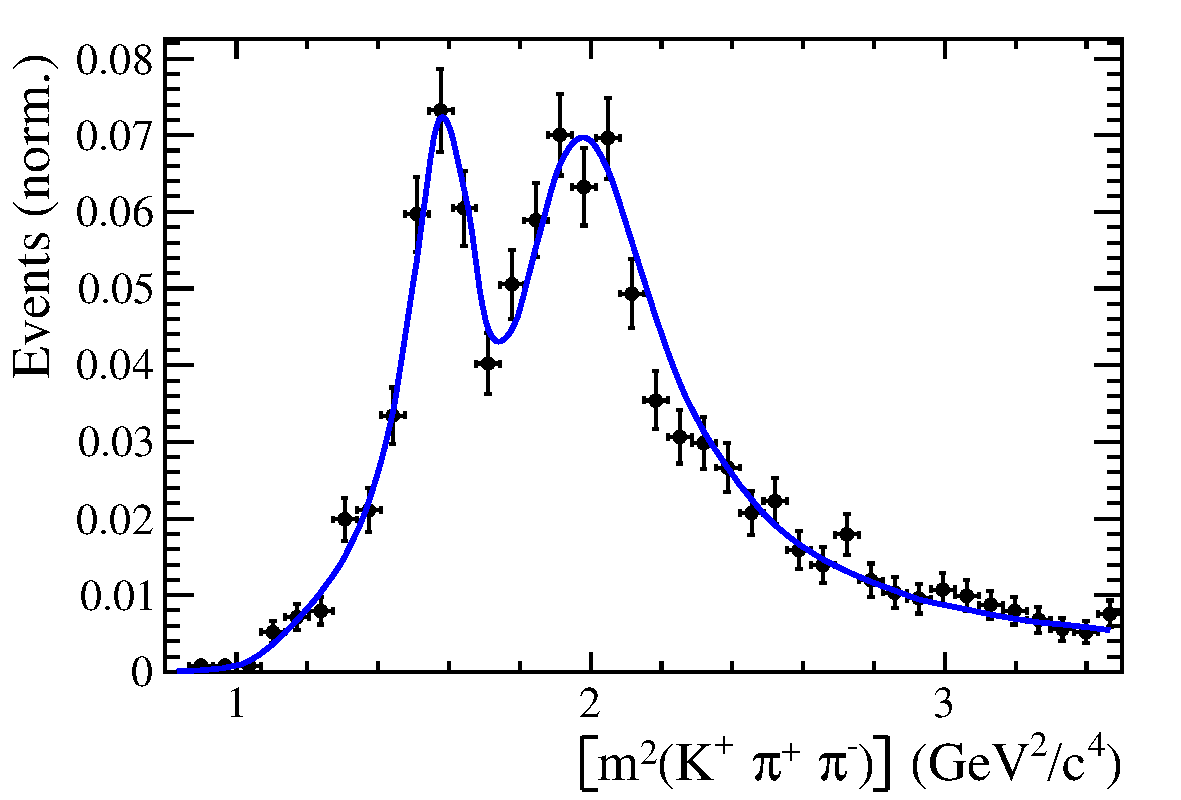
\includegraphics[width=0.35\textwidth, height = 3.cm]{plots_toys/s_Kpipi-eps-converted-to.pdf} 
		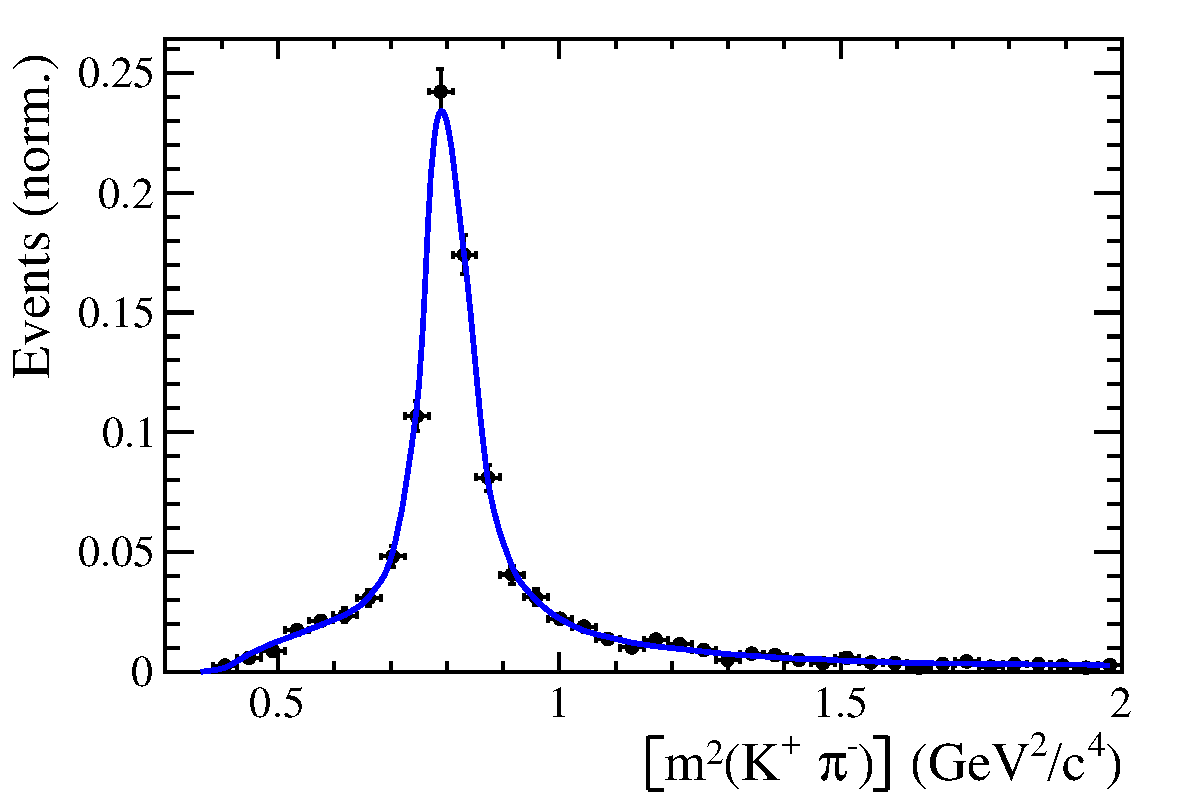
\includegraphics[width=0.35\textwidth, height = 3.cm]{plots_toys/s_Kpi-eps-converted-to.pdf} 
		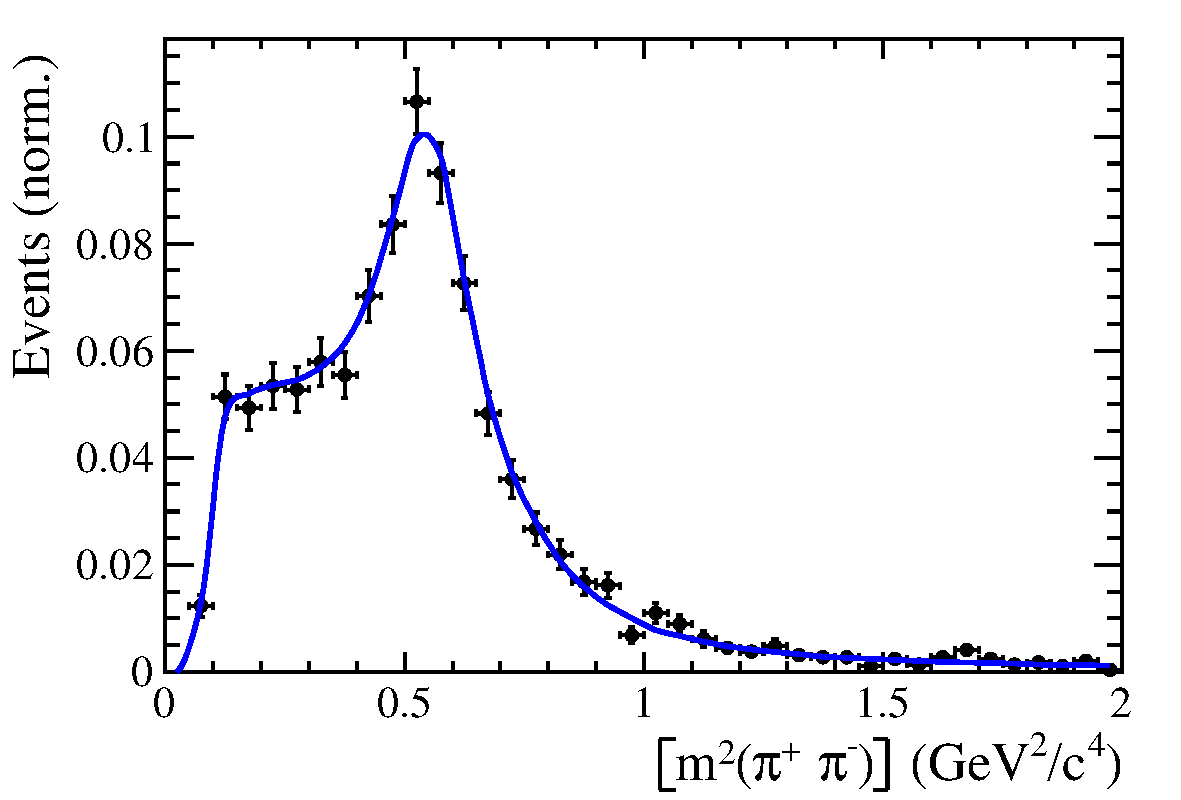
\includegraphics[width=0.35\textwidth, height = 3.cm]{plots_toys/s_pipi-eps-converted-to.pdf} 		
	\end{figure}				
\end{frame}


\appendix 
\addtocounter{framenumber}{-1} 

\begin{frame}
\thispagestyle{empty}
\bfseries\Huge

\begin{center}
Appendix
\end{center}

\normalfont

\end{frame}


\begin{frame}
\frametitle{Massfits norm 11}

\begin{figure}[h]
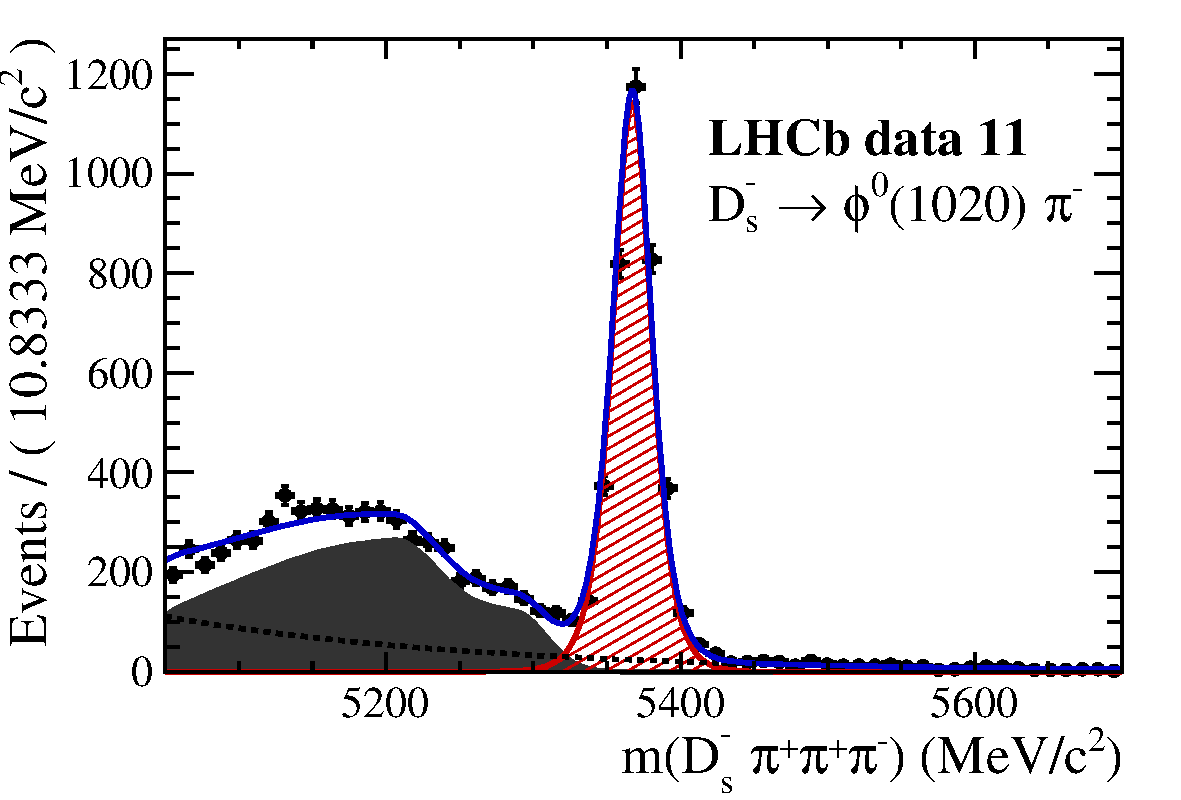
\includegraphics[height=!,width=0.5\textwidth]{plots/norm_y11_phipi.pdf}
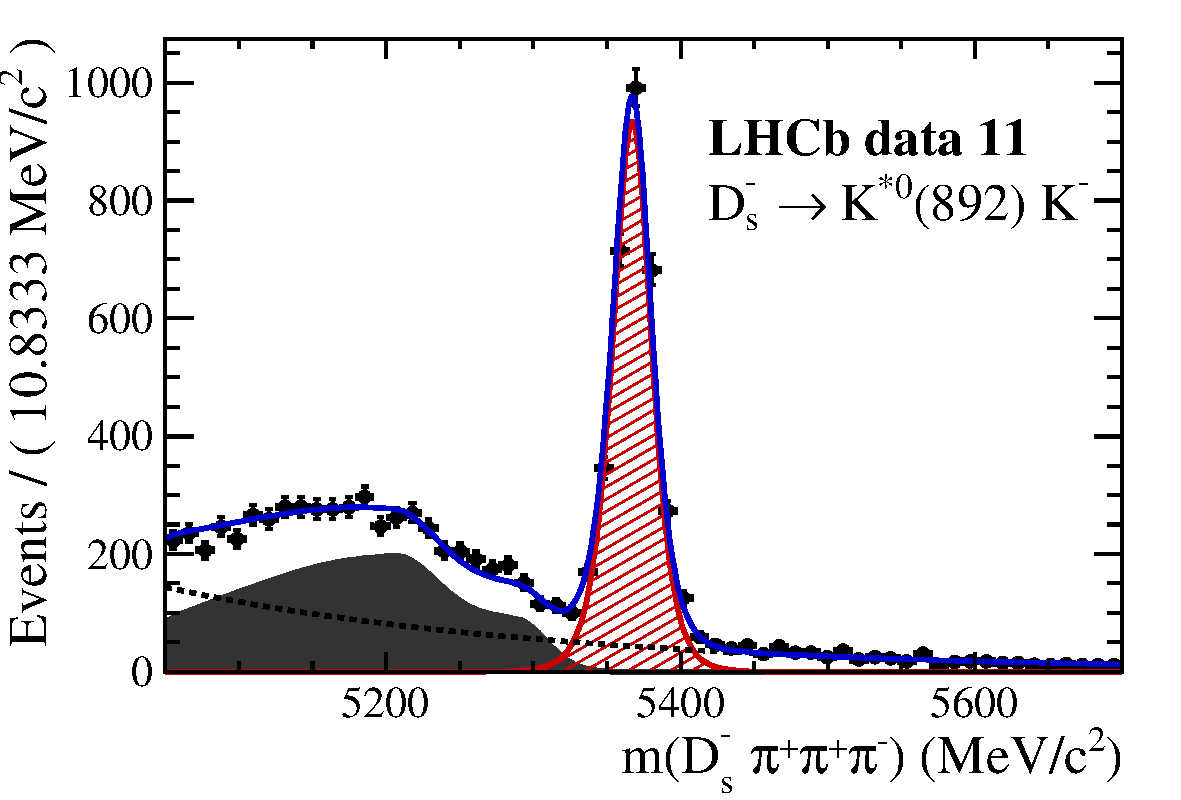
\includegraphics[height=!,width=0.5\textwidth]{plots/norm_y11_KsK.pdf}\\
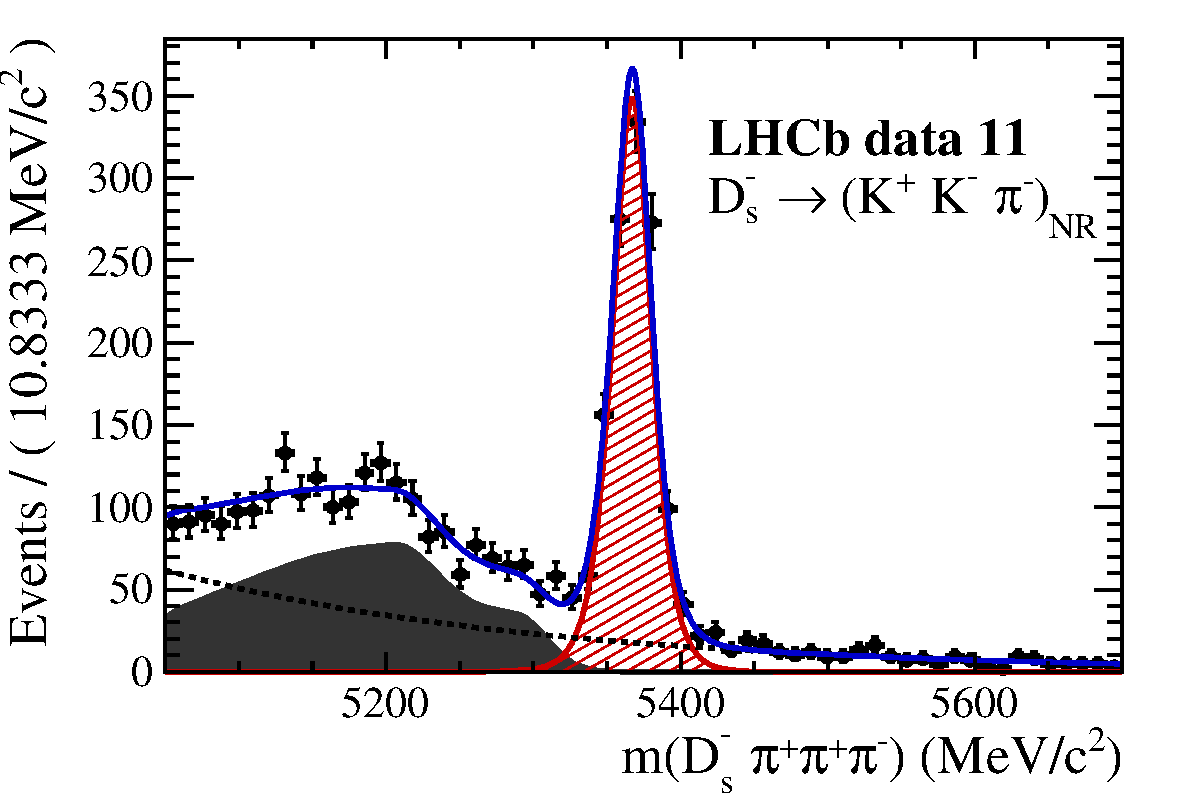
\includegraphics[height=!,width=0.5\textwidth]{plots/norm_y11_KKpi_NR.pdf}
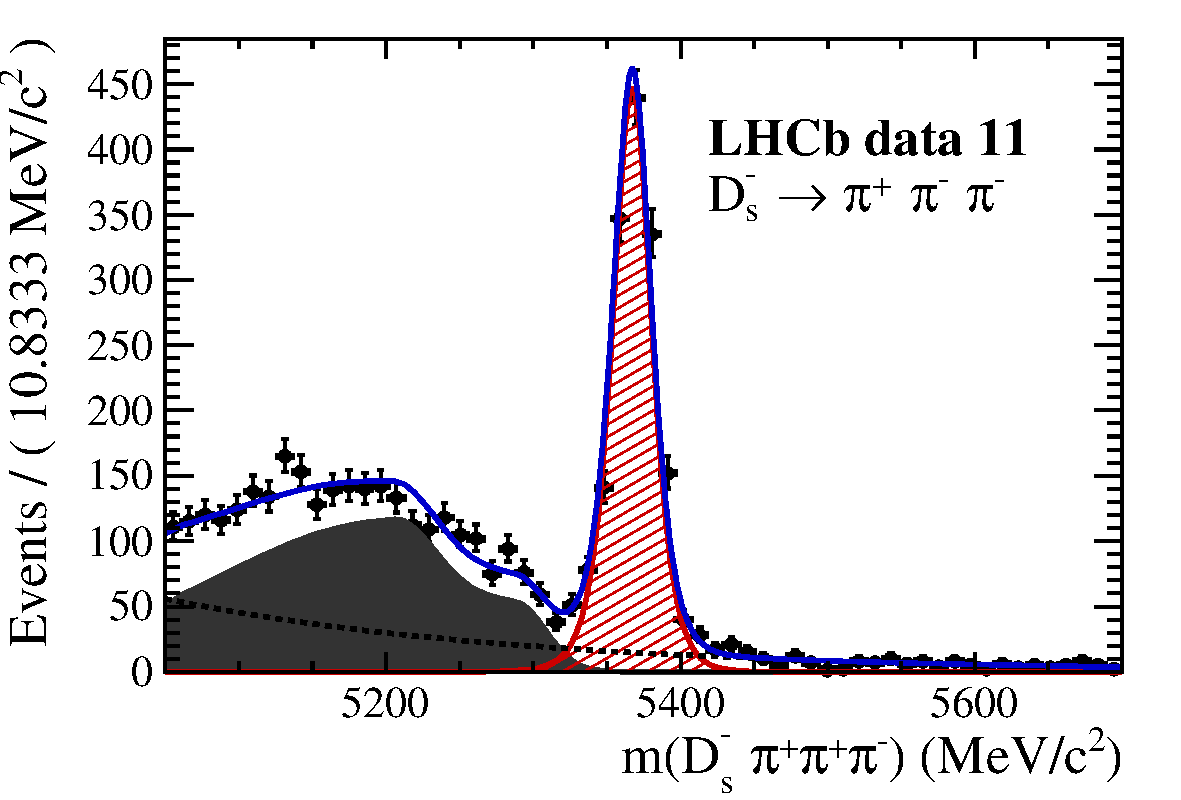
\includegraphics[height=!,width=0.5\textwidth]{plots/norm_y11_pipipi.pdf}
\end{figure}

\end{frame}

\begin{frame}
\frametitle{Massfits norm 12}

\begin{figure}
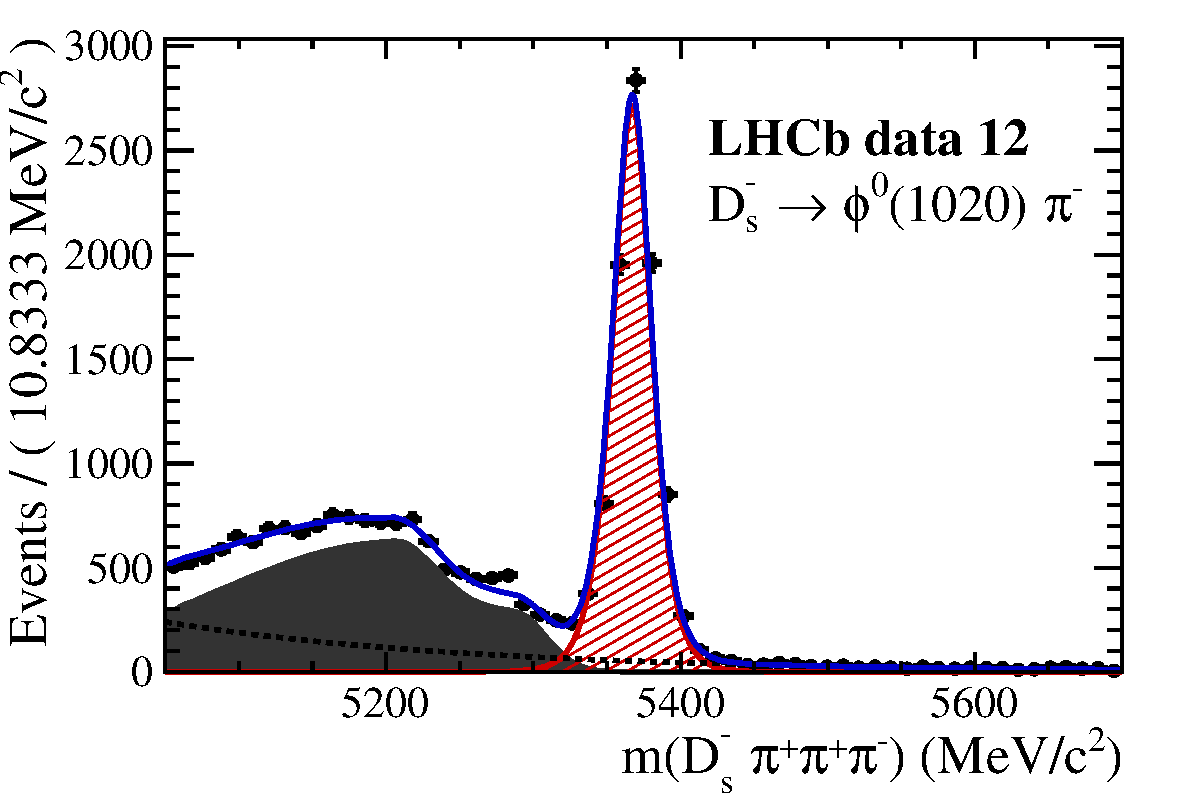
\includegraphics[height=!,width=0.5\textwidth]{plots/norm_y12_phipi.pdf}
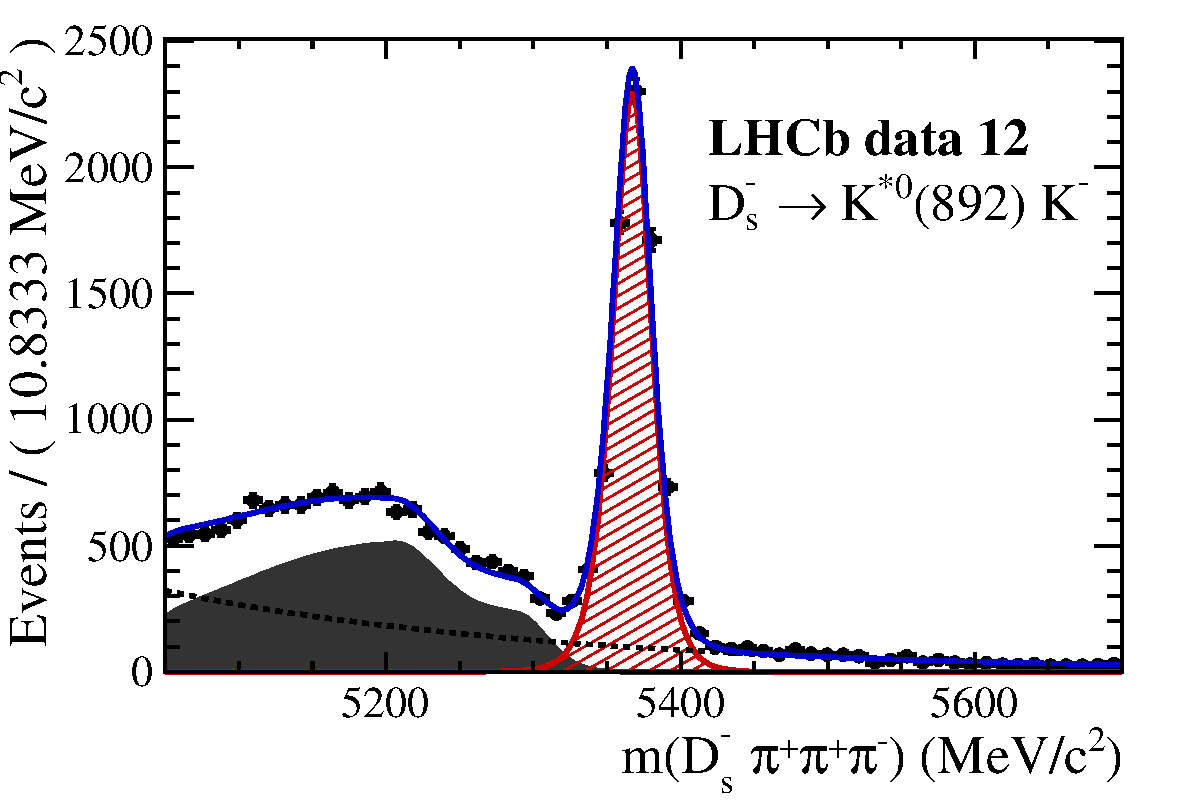
\includegraphics[height=!,width=0.5\textwidth]{plots/norm_y12_KsK.pdf}\\
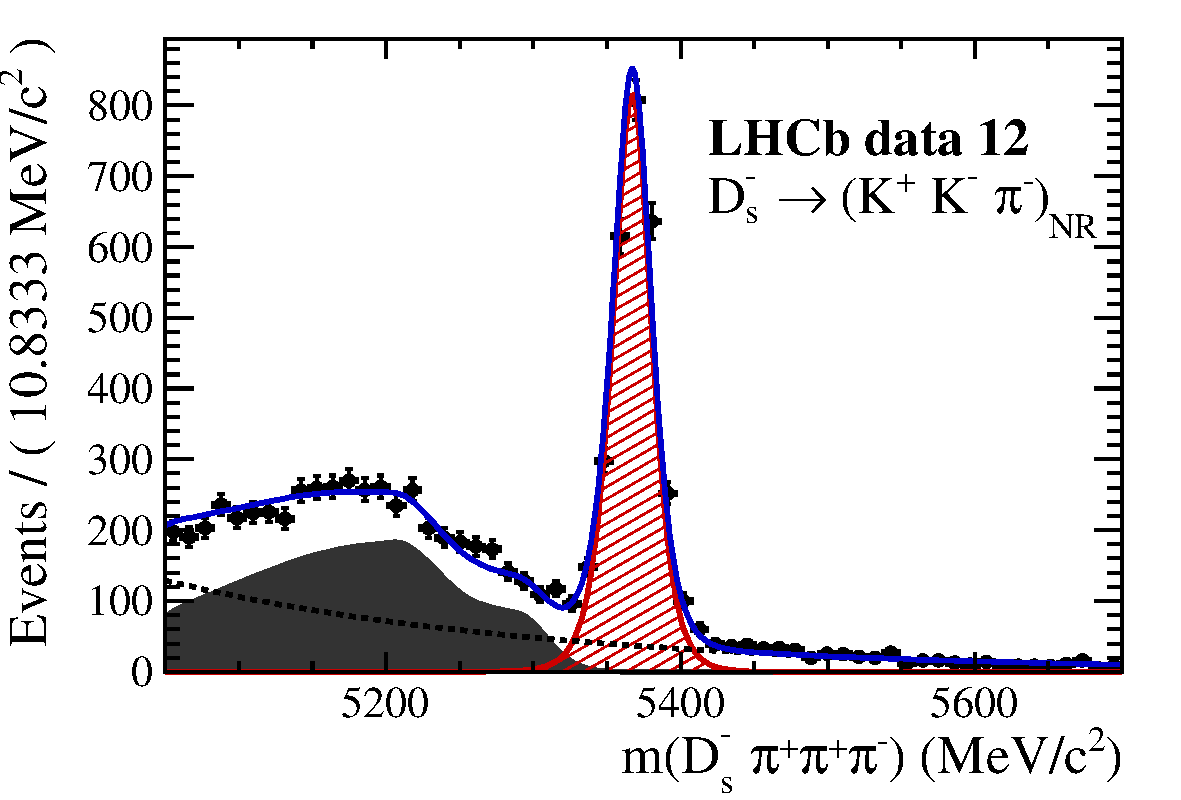
\includegraphics[height=!,width=0.5\textwidth]{plots/norm_y12_KKpi_NR.pdf}
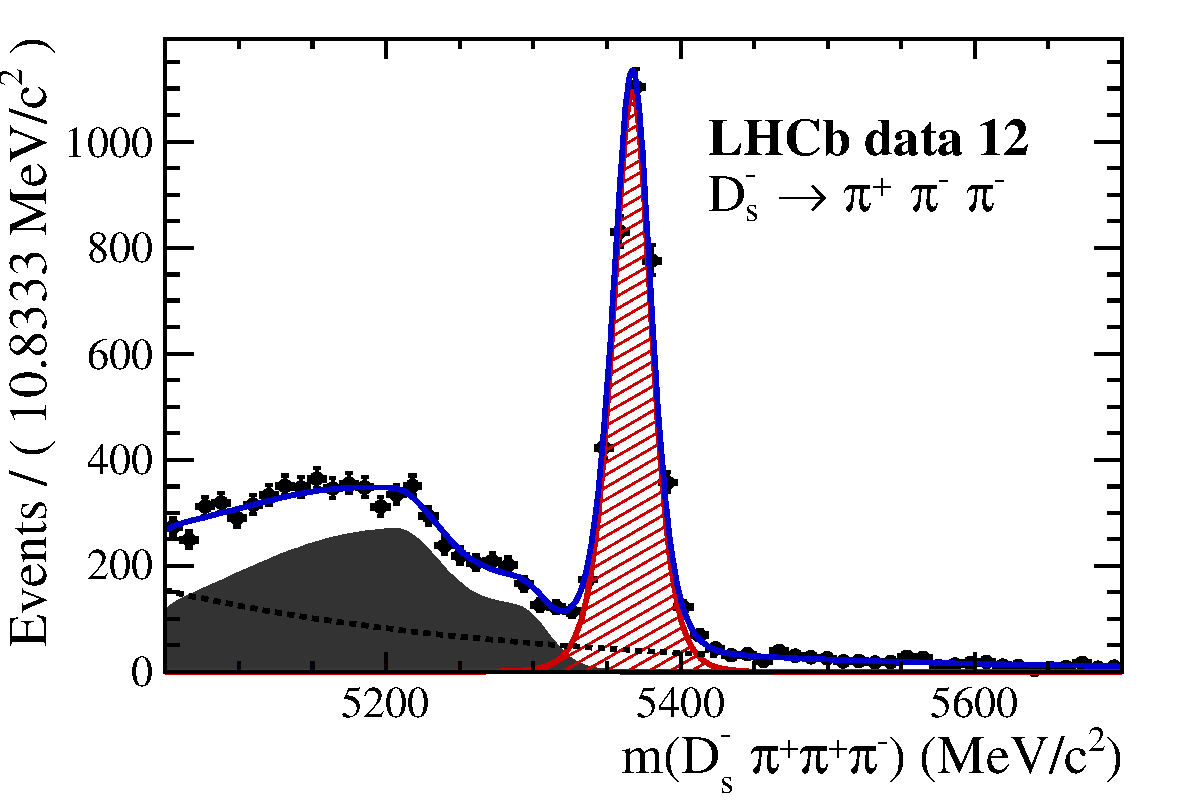
\includegraphics[height=!,width=0.5\textwidth]{plots/norm_y12_pipipi.pdf}
\end{figure}

\end{frame}

\begin{frame}
\frametitle{Massfits signal 11}

\begin{figure}[h]
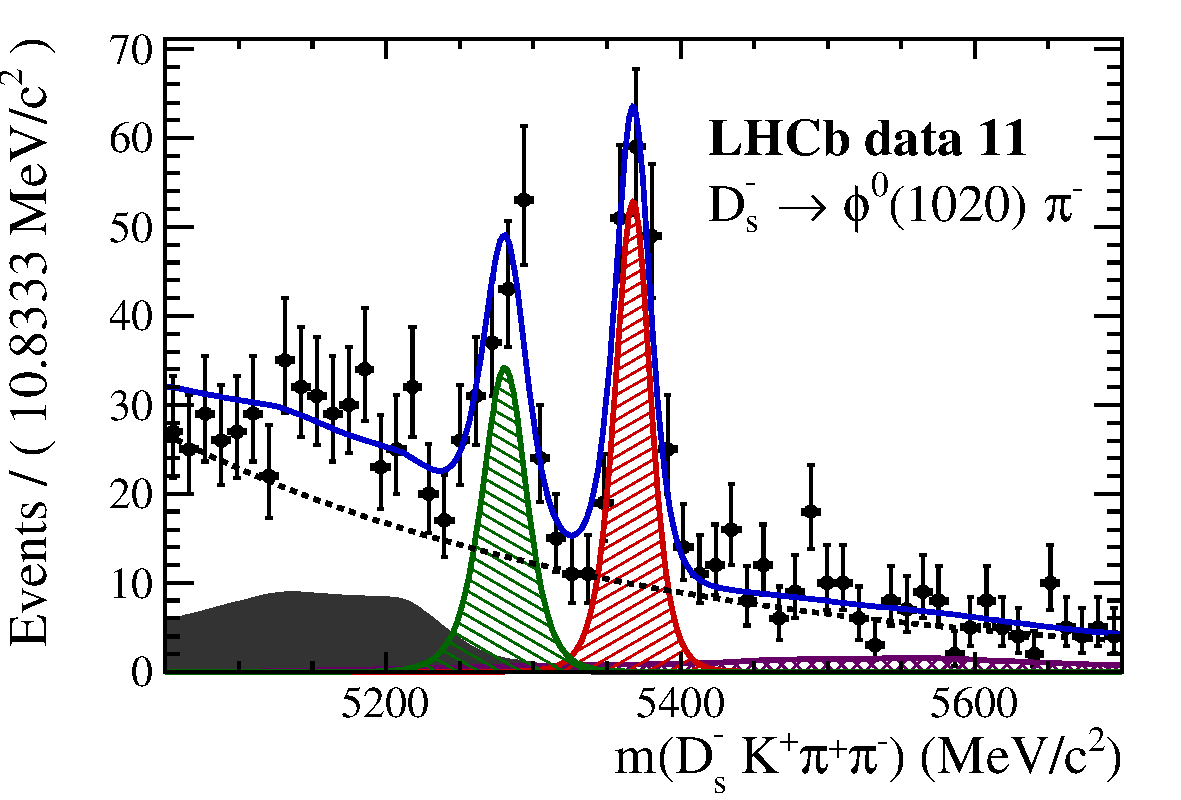
\includegraphics[height=!,width=0.5\textwidth]{plots/signal_y11_phipi.pdf}
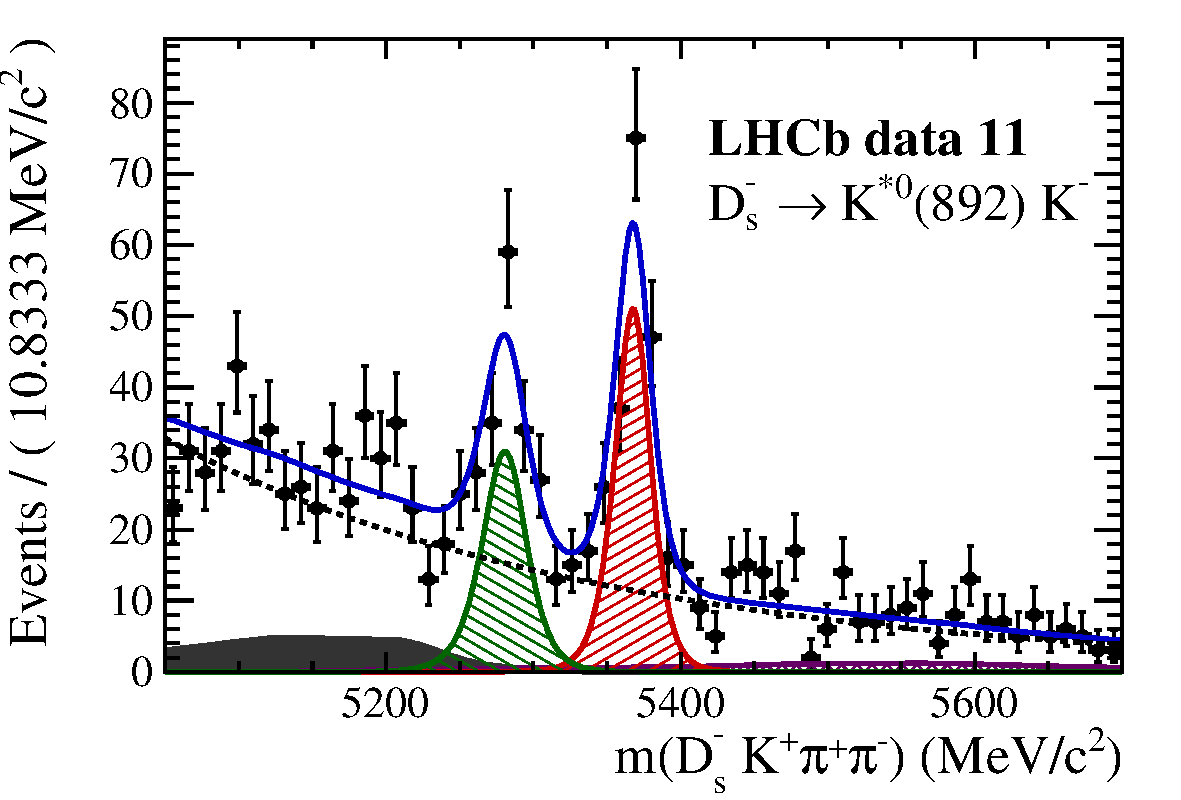
\includegraphics[height=!,width=0.5\textwidth]{plots/signal_y11_KsK.pdf}\\
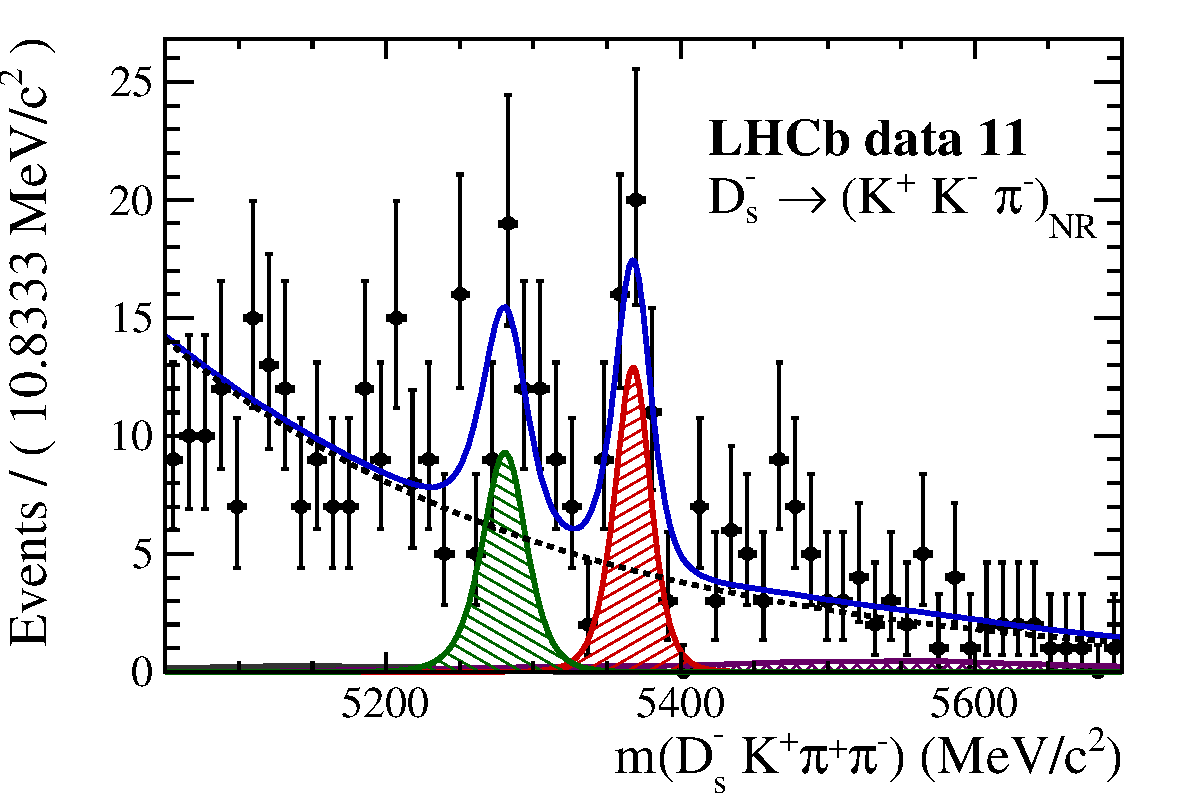
\includegraphics[height=!,width=0.5\textwidth]{plots/signal_y11_KKpi_NR.pdf}
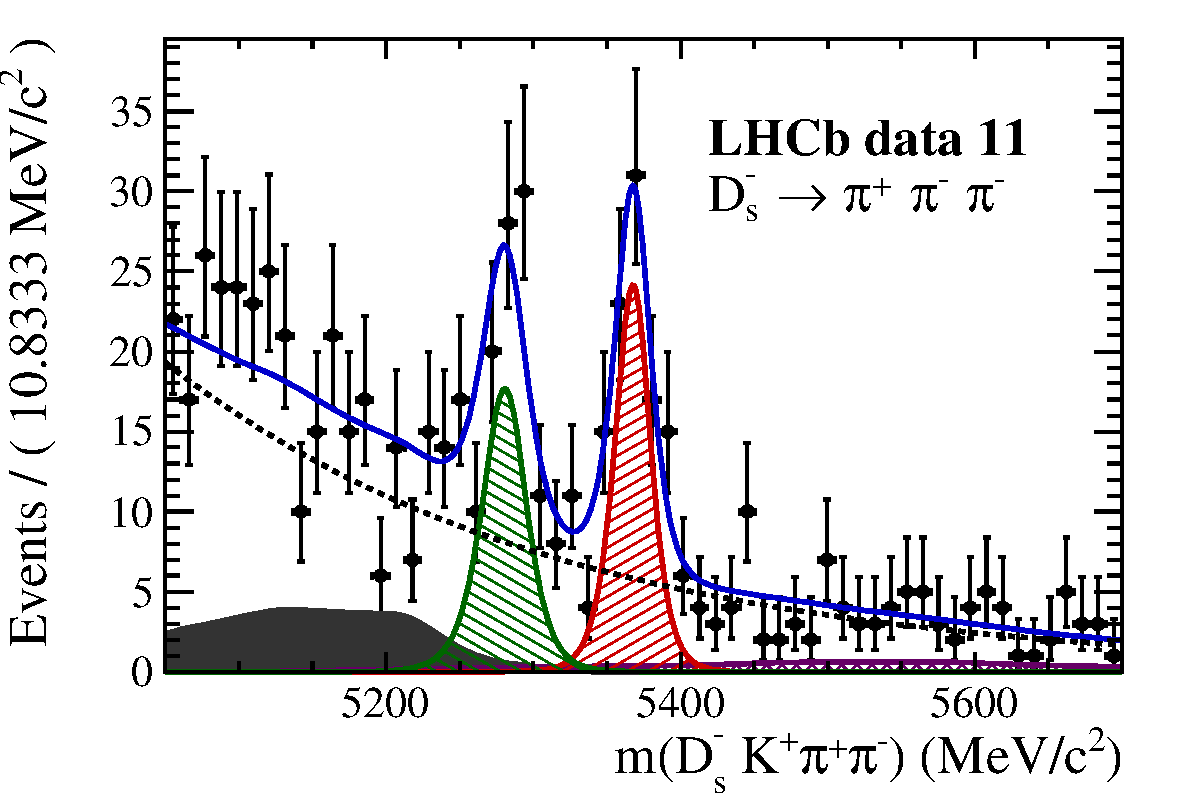
\includegraphics[height=!,width=0.5\textwidth]{plots/signal_y11_pipipi.pdf}
\end{figure}

\end{frame}

\begin{frame}
\frametitle{Massfits signal 12}

\begin{figure}
\includegraphics[height=!,width=0.5\textwidth]{plots/signal_y12_phipi.pdf}
\includegraphics[height=!,width=0.5\textwidth]{plots/signal_y12_KsK.pdf}\\
\includegraphics[height=!,width=0.5\textwidth]{plots/signal_y12_KKpi_NR.pdf}
\includegraphics[height=!,width=0.5\textwidth]{plots/signal_y12_pipipi.pdf}
\end{figure}

\end{frame}


\end{document}